%==============================================================================
% short introduction to get template running on WINDOWS
% further explanation can be found in the pptx
% can be removed after first compilation 
%
% install MikTeX (http://www.miktex.org) - activate auto-install of packages
% install ActivePerl (https://www.perl.org/) - add to HOME
% system reboot
%
% use command-line or IDE in admin-mode to execute the  following commands
% in the specified order (pdflatex used because we want the PDF in the end)
% 
%
% After changes in glossary you need to execute the following command 
% to use the new acronyms
%
% makeglossaries ma_mustermann
%
% After changes in literature you need to execute the following command
% to use the new reference
%
% bibtex ma_mustermann
%
%==============================================================================

% TODO set author and title in header settings

%==============================================================================
% Dokument einrichten und Pakete laden
%==============================================================================

\documentclass[
	pdftex,				% PDFTex verwenden da ausschliesslich ein PDF erzeugt wird.
	a4paper, twoside,	% Verwenden von DIN A4 Papier.
	11pt,				% Grosse Schrift, besser geeignet für A4.
	parskip=half,		% Halbe Zeile Abstand zwischen Absätzen.
	numbers=noenddot,	% Keine Punkte hinter Nummern
	pagesize,           % Schreibt die Papiergroesse in die Datei 
	BCOR=10mm,			% Bindekorrektur
	DIV=13,				% Alternativ 12 oder 14
	headinclude,		% Kopfzeile in den Textbereich
	headsepline,		% Linie nach Kopfzeile.
	openany,            % Keine leere Seite nach/vor neuem Kapitel
	titlepage,
	headings=small,
	bibliography=totocnumbered,	% Bibliographie im TOC nummeriert
]{scrbook}

\usepackage{setspace}\setstretch{1.2} 
%\usepackage{titlesec}

%\titlespacing\section{0pt}{12pt plus 4pt minus 2pt}{0pt plus 2pt minus 2pt}
%\titlespacing\subsection{0pt}{12pt plus 4pt minus 2pt}{0pt plus 2pt minus 2pt}
%\titlespacing\subsubsection{0pt}{12pt plus 4pt minus 2pt}{0pt plus 2pt minus 2pt}

%\usepackage{scrhack}

\usepackage[printonlyused]{acronym}
\usepackage{multicol}

%
% Zeichenkodieruung und Sprache
%

\usepackage[utf8]{inputenc} % Dokument
\usepackage[T1]{fontenc} % Schrift
\usepackage[ngerman, english]{babel}

%
% PDF-Metadaten setzen
%

\usepackage{pdfpages}
\usepackage[
	% Titel des PDF Dokuments
	% TODO set title
	pdftitle={git_manual},
	% Autor des PDF Dokuments
	% TODO set author
	pdfauthor={Anh Kha Nguyen},
	% Thema des PDF Dokuments
	pdfsubject={Git Manual: The subject-oriented approach},
	% Erzeuger des PDF Dokuments
	pdfcreator={Anh Kha Nguyen},
	% Schlüsselwörter für das PDF
	pdfkeywords={},
	% Dokumenttitel statt Dateiname anzeigen
	pdfdisplaydoctitle=true,																% Sprache des Dokuments
	pdflang=de,
	bookmarksopen=true,
	bookmarksdepth=1,
	colorlinks,
	linkcolor = black,
	citecolor=black,
	urlcolor=black,
]{hyperref}

%
%  Zusätzliche Pakete laden
%

% Anführungszeichen
\usepackage[style=american]{csquotes}

% erweiterte Tabelleneigenschaftn
\usepackage{array, ragged2e}

% Einbinden von Grafiken
\usepackage{graphicx}	

% mathematischer Textsatz
%\usepackage{amsmath}
%\usepackage{amssymb}
%\usepackage{dsfont}

% Textteile drehen
%\usepackage{rotating}	

% Farbpakete
%\usepackage{color}
%\usepackage{xcolor}

% Quellcode sauber formatieren
\usepackage{listings}	

% Font 'Latin Modern Family' verwenden
\usepackage{microtype}
\usepackage{helvet}
\usepackage{mathptmx}

%==============================================================================
% Einstellungen und Definitionen
%==============================================================================

% Farben definieren

\definecolor{light-gray}{gray}{0.95}
%\definecolor{LinkColor}{rgb}{0,0,0.5}
%\definecolor{ListingBackground}{rgb}{0.85,0.85,0.85}
%\definecolor{CommentColor}{rgb}{0, 0.5, 0}
%\definecolor{StringColor}{rgb}{0.63, 0.09, 0.09}

% KOMA-Script Option, Zeilenumbruch bei Bildbeschreibungen.
\setcapindent{1em}

% Stil der Kopf- und Fusszeilen.
\usepackage[headsepline,automark,pagestyleset=KOMA-Script,markcase=ignoreuppercase]{scrlayer-scrpage}
\pagestyle{scrheadings}

% Stil der Überschriften auf normale Schrift.

%\setkomafont{sectioning}{\normalfont\bfseries}		 % Titel mit Normalschrift
\setkomafont{captionlabel}{\normalfont\bfseries}	 % Fette Beschriftungen 
%\setkomafont{pageheadfoot}{\normalfont\itshape}     % Kursive Seitentitel
\setkomafont{descriptionlabel}{\normalfont\bfseries} % Fette Beschreibungstitel

% Codelisting korrekt bezeichnet ausgeben
\renewcommand\lstlistingname{Source Code}

%==============================================================================
% Listings
%==============================================================================

\lstloadlanguages{% Check Dokumentation for further languages ...
  XML,
  HTML,
  Java,
  Tex
}


\lstset{
  %basicstyle=\scriptsize\ttfamily, % Standardschrift
	basicstyle=\footnotesize\ttfamily,
  %numbers=left, % Ort der Zeilennummern
  %numberstyle=\tiny, % Stil der Zeilennummern
  %stepnumber=2, % Abstand zwischen den Zeilennummern
	%numberblanklines=false,
  numbersep=5pt, % Abstand der Nummern zum Text
  tabsize=2, % Groesse von Tabs
  extendedchars=true, %
  breaklines=true, % Zeilen werden Umgebrochen
  %keywordstyle=\color{red},
  frame=b,
  % keywordstyle=[1]\textbf, % Stil der Keywords
  % keywordstyle=[2]\textbf, %
  % keywordstyle=[3]\textbf, %
  % keywordstyle=[4]\textbf, \sqrt{\sqrt{}} %
  %stringstyle=\color{white}\ttfamily, % Farbe der String
  showspaces=false, % Leerzeichen anzeigen ?
  showtabs=false, % Tabs anzeigen ?
  xleftmargin=17pt,
	xrightmargin=17pt,
  framexleftmargin=17pt,
  framexrightmargin=17pt,
  framexbottommargin=4pt,
  backgroundcolor=\color{white},
  showstringspaces=false % Leerzeichen in Strings anzeigen ?
}

\lstset{literate=%
    {Ö}{{\"O}}1
    {Ä}{{\"A}}1
    {Ü}{{\"U}}1
    {ß}{{\ss}}1
    {ü}{{\"u}}1 
    {ä}{{\"a}}1
    {ö}{{\"o}}1
    {~}{{\textasciitilde}}1
}

\usepackage{caption}
\DeclareCaptionFont{white}{\color{white}}
\DeclareCaptionFormat{listing}{\colorbox[cmyk] {0.43, 0.35, 0.35,0.01}{\parbox{\textwidth-2\fboxsep-2\fboxrule-0pt} {\hspace{15pt}#1#2#3}}}
\captionsetup[lstlisting]{format=listing,labelfont=white, textfont=white,singlelinecheck=false, margin=0pt, font={bf,footnotesize}}

%
% code listing style
%

\lstdefinestyle{kit-cm}{
  backgroundcolor=\color{light-gray},
  belowcaptionskip=1\baselineskip,
  breaklines=true,
  frame=single,
  framexleftmargin=15pt,
  language=C,
  showstringspaces=false,
  basicstyle=\footnotesize\ttfamily, 
  numbers=left,                    
  numbersep=7pt,                
  numberstyle=\tiny\color{black},
  captionpos=b
}

\lstdefinelanguage{Swift}{
  keywords={associatedtype, class, deinit, enum, extension, func, import, init, inout, internal, let, operator, private, protocol, public, static, struct, subscript, typealias, var, break, case, continue, default, defer, do, else, fallthrough, for, guard, if, in, repeat, return, switch, where, while, as, catch, dynamicType, false, is, nil, rethrows, super, self, Self, throw, throws, true, try, associativity, convenience, dynamic, didSet, final, get, infix, indirect, lazy, left, mutating, none, nonmutating, optional, override, postfix, precedence, prefix, Protocol, required, right, set, Type, unowned, weak, willSet},
  ndkeywords={class, export, boolean, throw, implements, import, this},
  sensitive=false,
  comment=[l]{//},
  morecomment=[s]{/*}{*/},
  morestring=[b]',
  morestring=[b]"
}

\lstdefinelanguage{Gherkin}{
	morekeywords = {
		Given,
		When,
		Then,
		And,
		Scenario,
		Feature,
		But,
		Background,
		Scenario Outline,
		Examples
	},
	sensitive=true,
	morecomment=[l]{\#},
	morestring=[b]",
	morestring=[b]'
}

\lstdefinelanguage{json}{
     string=[s]{"}{"},
    stringstyle=\color{blue},
    comment=[l]{:},
    commentstyle=\color{black},
}

\DeclareCaptionFont{black}{\color{black}} 
\DeclareCaptionFormat{listing}
  {\colorbox{white}
     {\parbox{\dimexpr\textwidth-2\fboxsep}{\centering #1#2#3}}}
\captionsetup[lstlisting]{format=listing,labelfont=black,textfont=black}

\usepackage{hyperref}
\usepackage{paralist}
\usepackage{subcaption}
\usepackage{booktabs}
\usepackage{listings}
\usepackage{caption}

%
% todo notes
%

\usepackage{todonotes}
%\usepackage[disable]{todonotes}	% hide all todo notes
%\presetkeys{todonotes}{inline}{}	% show all defined todos as inline

%
% glossary
%

\usepackage[acronym,numberedsection]{glossaries}
\setacronymstyle{long-short}
%\loadglsentries{chapters/glossar}
\loadglsentries{git_manual/chapters/glossar.tex}
\makeglossaries

%
% load additional packages
%

\usepackage{calc}
\usepackage{enumitem}
\usepackage{multirow}
\usepackage{mathtools}
\usepackage{enumitem}
\usepackage{amsmath} 
\usepackage{amssymb}
\usepackage{wasysym}
\usepackage{rotating}
\usepackage{pgfplots}
\usepackage{longtable}
\usepackage{algorithm}
\usepackage{algpseudocode}
\usepackage{float}
\usepackage{pdfpages}
\usepackage{threeparttablex}
\usepackage{longtable,lscape}
\usepackage{tablefootnote}
\usetikzlibrary{patterns}
\usepackage{multicol}
\usepackage{bm}
\usepackage{esvect}
%\usepackage{subfigure}
\floatname{algorithm}{Algorithmus}

\makeindex

\usepackage{bera}% optional: just to have a nice mono-spaced font
\usepackage{listings}
\usepackage{xcolor}

\colorlet{punct}{red!60!black}
\definecolor{background}{HTML}{EEEEEE}
\definecolor{delim}{RGB}{20,105,176}
\colorlet{numb}{magenta!60!black}

\usepackage{tabularx}

\usepackage{listingsutf8}

\pretocmd{\chapter}{\glsresetall}{}{}

\begin{document}

%==============================================================================

%
% add title pages
%

\frontmatter
\setcounter{secnumdepth}{3}
\begin{titlepage}
\thispagestyle{empty}
\enlargethispage{2cm}
%\enlargethispage{\baselineskip}

\sffamily
%\centering
\vspace*{-3.2cm}
\hspace*{-0.6cm}
\begin{figure}
    \begin{subfigure}[b]{0.3\textwidth}
         \centering
         
\includegraphics[height=2.14cm]{figures/kit-logo}
     \end{subfigure}
     \begin{subfigure}[b]{0.3\textwidth}
         \centering
         
\includegraphics[height=2.14cm]{git_manual/figures/imi.pdf}
     \end{subfigure}
\end{figure}

\begin{addmargin}{2cm}

\vfill

\begin{tabular}{>{\RaggedRight}p{12cm}}
	{\textbf{\huge Git Manual: The Subject-Oriented Approach}}\\
	\\
	\\
	{Author: Anh Kha Nguyen }  \\
	{Semester: 7. Bachelor Semester } \\
	{Supervisor: Dr.-Ing. Dipl.-Wi.-Ing. Matthes Elstermann} \vspace{2em} \\
	\\
	{\LARGE }
\end{tabular}
\vfill
\vfill
\vfill


%\singlespacing

\vspace{1em}
\begin{tabular}{ll}
	

	Winter Semester 2020 \\
	\\
	\multicolumn{2}{l}{Institute for Information Management and Engineering} \\
	\multicolumn{2}{l}{www.imi.kit.edu} \\
	\\
	\multicolumn{2}{l}{\scriptsize{KIT - The Research University in the Helmholtz Association}}\\
\end{tabular}

\end{addmargin}
\newpage
\thispagestyle{empty}
\end{titlepage}	% TODO set author and title

\tableofcontents
%
% add content
%


\mainmatter
%\glsresetall
\chapter{Introduction}
\label{cha:introduction}
This chapter gives a brief overview of the the document's overall motivation, its current state and the needed background knowledge that is required to read this document.

\section{Motivation and current state}
As the title suggests, the document's overall motivation is to deliver a subject-oriented approach of a git manual.
Git is a Version Control System (VCS) developed by Linus Torvalds \cite{LM12}. Compared to other VCSs, The main difference of git is that it has a different approach to file versioning and collaboration development, as both are much more efficient in git \cite{CS20}.
This makes git one of the most popular VCS out there, which is why the provision of git instruction is of particular interest.
The end goal of this document is to provide the \textit{ultimate} git manual. Its final version should aspire to provide all the necessary knowledge about git to any reader, regardless of his/her technical background.

As of the document's current state, it provides 12 git commands which lay a solid foundation for any basic git workflow. With the provided commands, the reader is able to: 
\begin{itemize} [nosep]
    \item \textbf{create} a git repository (\ref{sec:git_init})
    \item \textbf{add} (\ref{sec:git_add}) and \textbf{commit} (\ref{sec:git_commit}) any file within a git repository
    \item \textbf{check the current state} of a git repository at any given time (\ref{sec:git_status})
    \item \textbf{view} all existing branches and \textbf{create} new ones (\ref{sec:git_branch})
    \item \textbf{switch} to any existing branch (\ref{sec:git_checkout})
    \item \textbf{merge} different branches of a git repository (\ref{sec:git_merge})
    \item \textbf{set a new branch beginning} for any branch of a git repository (\ref{sec:git_rebase})
    \item \textbf{save} a copy of a remote git repository into the local storage (\ref{sec:git_clone})
    \item \textbf{fetch} commits of a remote repository (\ref{sec:git_fetch})
    \item \textbf{pull} (fetch and apply) commits of a remote repository on any branch (\ref{sec:git_pull})
    \item \textbf{push} commits of any branch of a repository to its local counterpart (\ref{sec:git_push})
\end{itemize}
This set of commands is enough for the majority of git workflows as the conjunction of all commands enables the usage of git's VCS functionality (\ref{cha:git_basics}), as well as the basic functionalities of branching (\ref{cha:git_branching}) and collaborations (\ref{cha:git_collaboration}).

\section{Foundations and related work}
There are three concepts that are required to fully understand this manual. The first concept is that git has introduced three different states for a file residing in a git repository.
\begin{figure} [H]
    \centering
    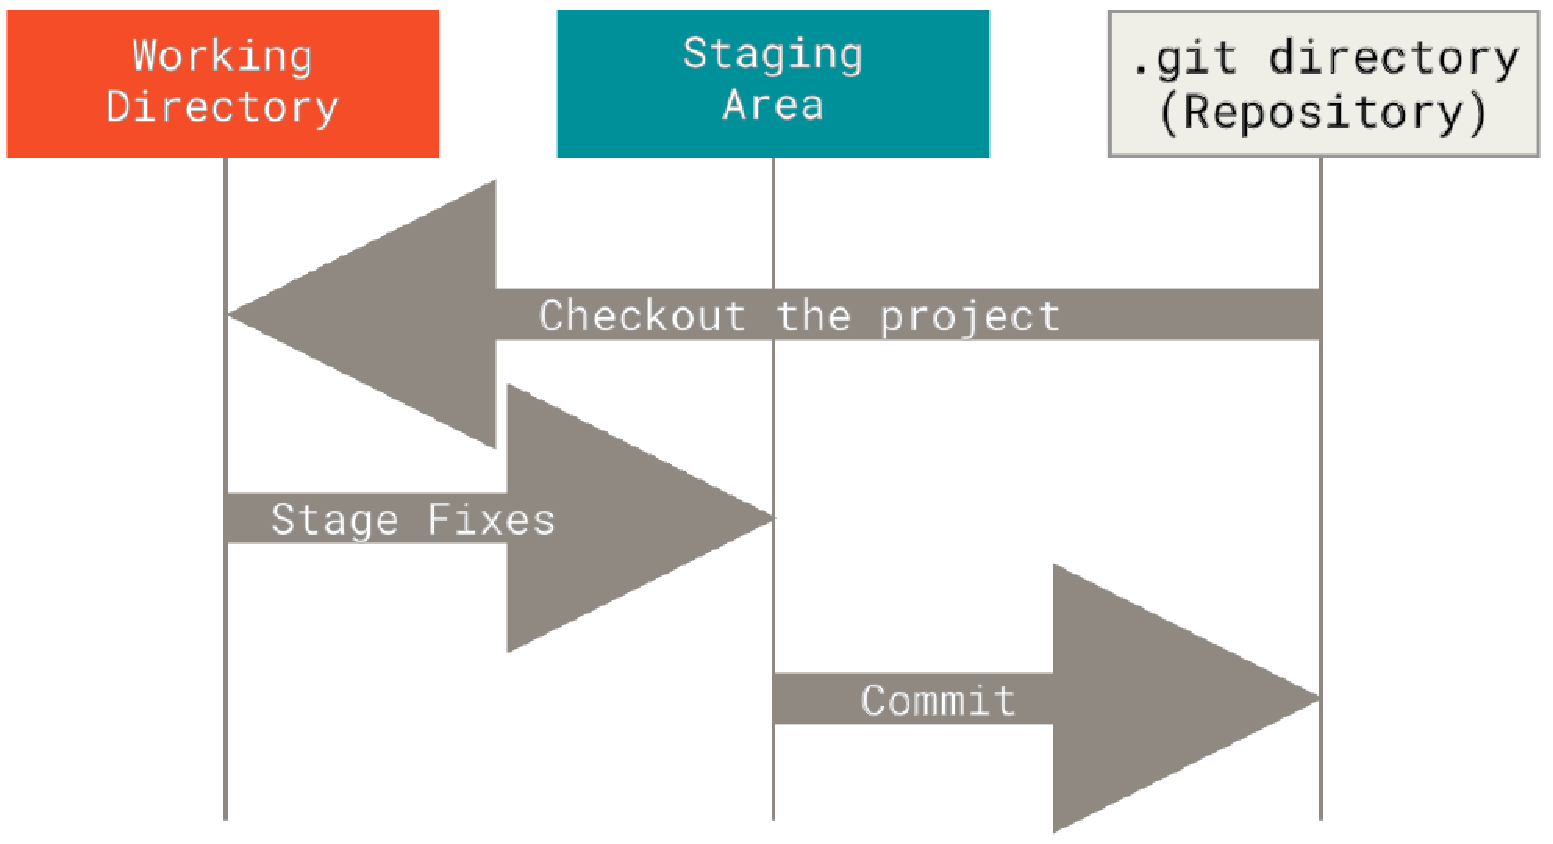
\includegraphics[width=\textwidth]{git_manual/figures/three_states.pdf}
    \caption{These are the transitions that happen in a state change\cite{CS20}}
    \label{fig:three_states}
\end{figure}
The three states are: \textit{modified}, \textit{staged} and \textit{committed}. If a file is modified, it means that the file has been changed or worked on, but is not committed yet.
To do that, the file has to be staged first. This means that the modified file is marked to go into the next commit. The file which keeps track of the marked files is called the \dq{}index\dq{}. If the user commits the staged file, the file is in its committed state which means that the data, containing the changes, is safely stored in the git repository

As seen in \ref{fig:three_states}, there are three locations the files can be in during the work with a git repository: the \textit{working directory}, \textit{staging area} and \textit{.git directory}. This is the second concept to remember during the read of the manual.
By opening any file within a git repository, git will automatically checkout the latest version of the project by translating and putting the compressed files within the repository onto the local disk. These modified files will then go through the three states depending on the workflow.

The third concept is completely unrelated to git and revolves around the process modeling schema itself. In the scope of this document, the Parallel Activity Specification Schema (PASS) is used to give a subject-oriented perspective of what process are involved during the interaction of a git user and the git software. Both are used as the main subjects of all Subject Interaction Diagrams (SID). Each git command has at least one SID. More details about PASS and its properties are found here \cite{El21}.
Here are some detailed descriptions of the main subjects:
\begin{itemize} [nosep]
    \item \textbf{Git User}: The Git User is the user of the git software.
    \item \textbf{Git UI + Software}: The Git UI could be the terminal of the user's current operating system or a graphical user interface written by a third party, such as GIT Bash. The git software is the actual part, which is installed in the user's computer. It contains all the logical operations required for the git commands.
\end{itemize}

\section{Outlook}
This is a list of git commands that are still left to model to complete the git manual in such a way so that its completed. However, this list does not contain every git command that is missing as each git command is heavily overloaded. An intrinsically complete manual is not only confusing, but unnecessary too as some overloaded git commands can be replaced with a sequence of other git commands.
\begin{itemize} [nosep]
    \item git config - Used to setup a profile for the git user, who contributes something to the 
    \item .gitignore: not a git command. However, it is important for the setup as the file is used to ignore unrelated files from the repository, e.g., .DS\_Store
    \item git diff: To see what has been modified which hasn't been staged yet
    \item git rm: removes a file from the git repository
    \item git log: views all commits
    \item git branch -d and git branch -D: deletes the targeted branch
    \item git cherry-pick: take a commit from a different branch and reintroduce it as new commit in the current branch
    \item git revert: take a commit from the current branch, remove it and introduce the removal as new commit. This essentially undoes the changes of the targeted commit.
    \item git stash: saves modified files on the computers stack. This is not a commit.
    \item git stash apply: Applies the modifications stored in the stash on the current branch again
    \item git stash list: Lists out all of the applicable stashes.
    \item git stash drop: Deletes the stashed modification from the stack.
    \item git reset: resets the HEAD pointer to a specific state.
    \item git push --set-upstream: pushes branches that are non existent in the remote repository into the remote repository.
\end{itemize}
After this list of commands is modeled completely, almost every functionality of git is unlocked and supported by this manual. The commands, which are intentionally left out, are rarely used even by professional software developers. However, if a git expert considers some commands missing, please refer to \cite{CS20} for guidance.
\chapter{Git Basics}
\label{cha:git_basics}
This chapter has every git command related to the basic VCS functionalities. After completing this chapter, the reader will be able to initialize and setup his own git repository, do basic versioning via committing changes and view the current status of the reader's current working directory.

\textit{Additional Information}: The git software uses a so-called \dq{}HEAD\dq{}-pointer to point at the latest commit of the git repository. So if a new commit is done, the HEAD will be updated to point at the new commit. Every commit points to its previous commit. An illustration of this is seen in (\ref{fig:branch_pointer}).

\newpage

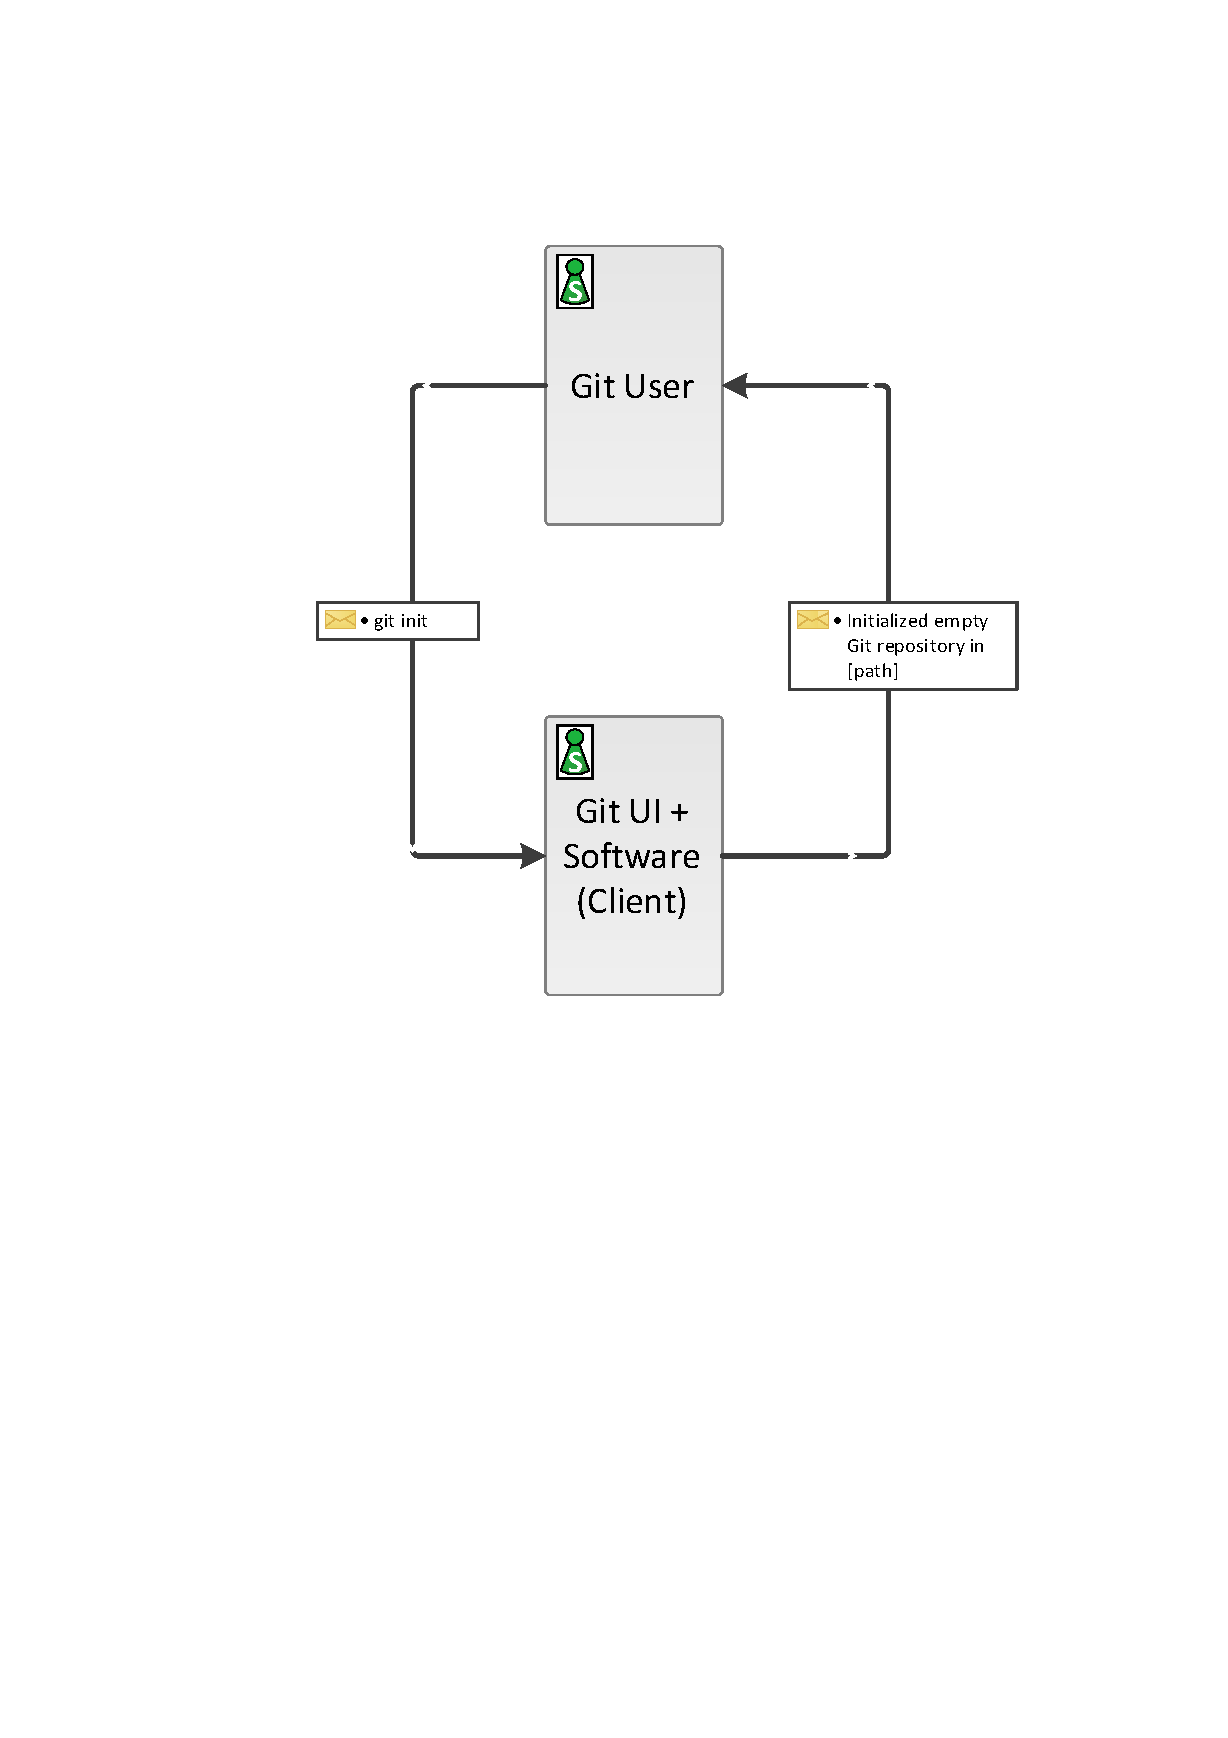
\includepdf[pages=1,pagecommand= {\section{git init} \label{sec:git_init}},scale=0.9]{git_commands/git_init.pdf}
\includepdf[pages=2-last,pagecommand={} ,scale=0.8]{git_commands/git_init.pdf}

\newpage

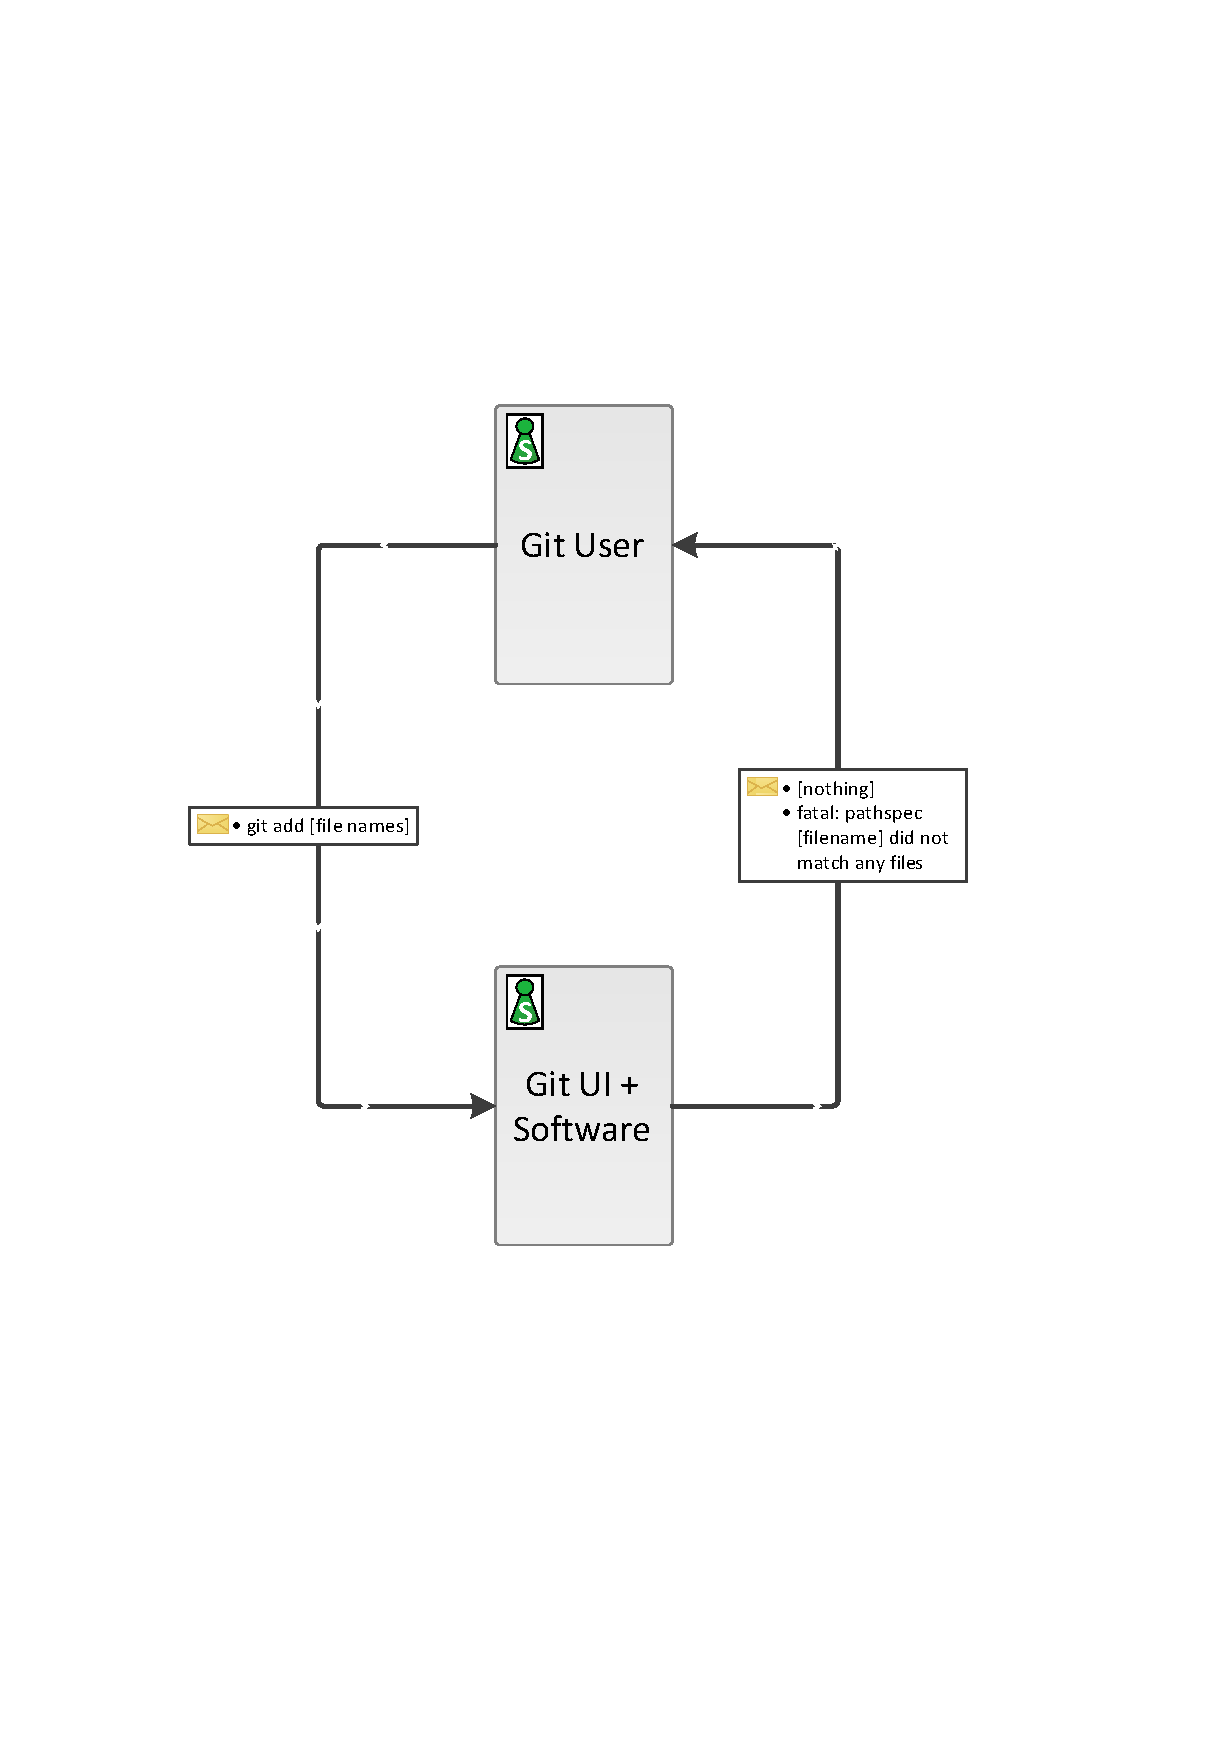
\includepdf[pages=1,pagecommand= {\section{git add} \label{sec:git_add}},scale=0.9]{git_commands/git_add.pdf}
\includepdf[pages=2-last,pagecommand={} ,scale=0.8]{git_commands/git_add.pdf}

\newpage

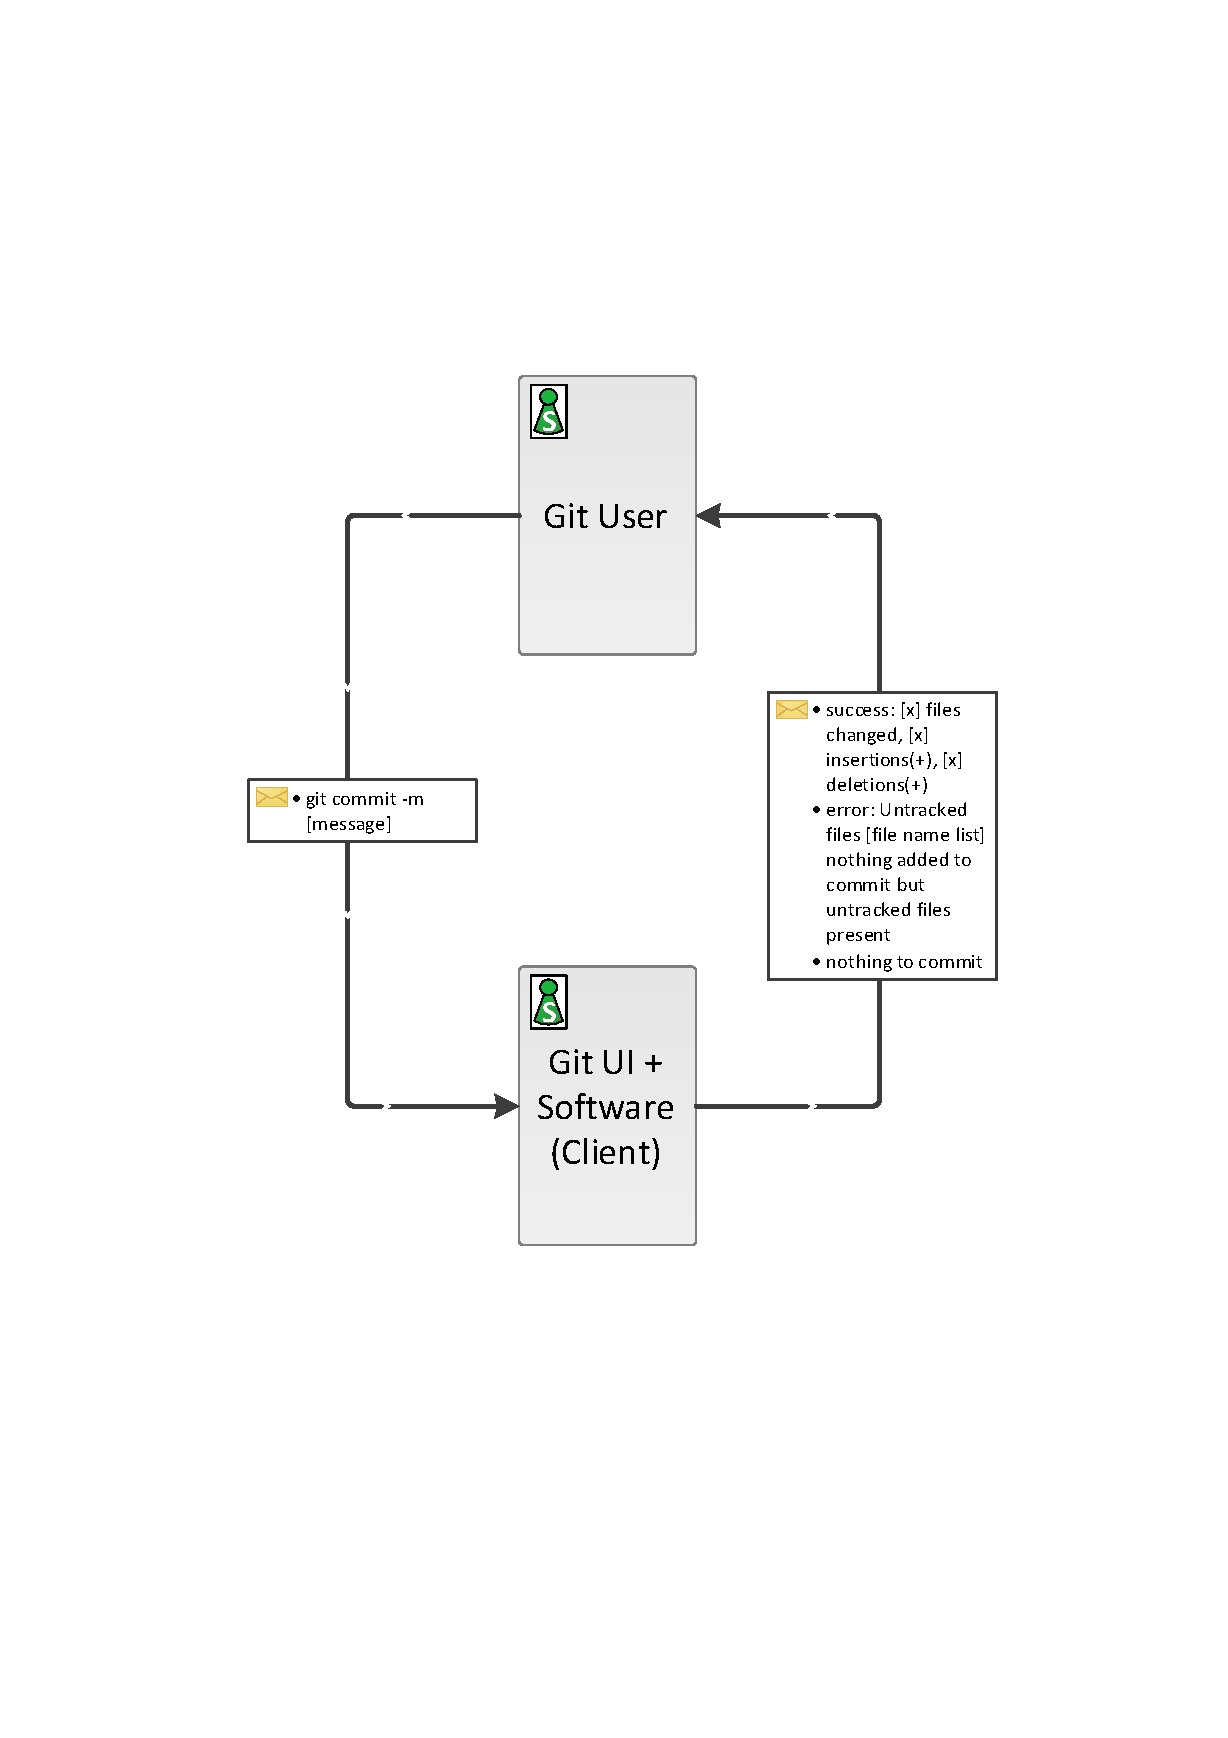
\includepdf[pages=1,pagecommand= {\section{git commit} \label{sec:git_commit}},scale=0.9]{git_commands/git_commit.pdf}
\includepdf[pages=2-last,pagecommand={} ,scale=0.8]{git_commands/git_commit.pdf}

\newpage

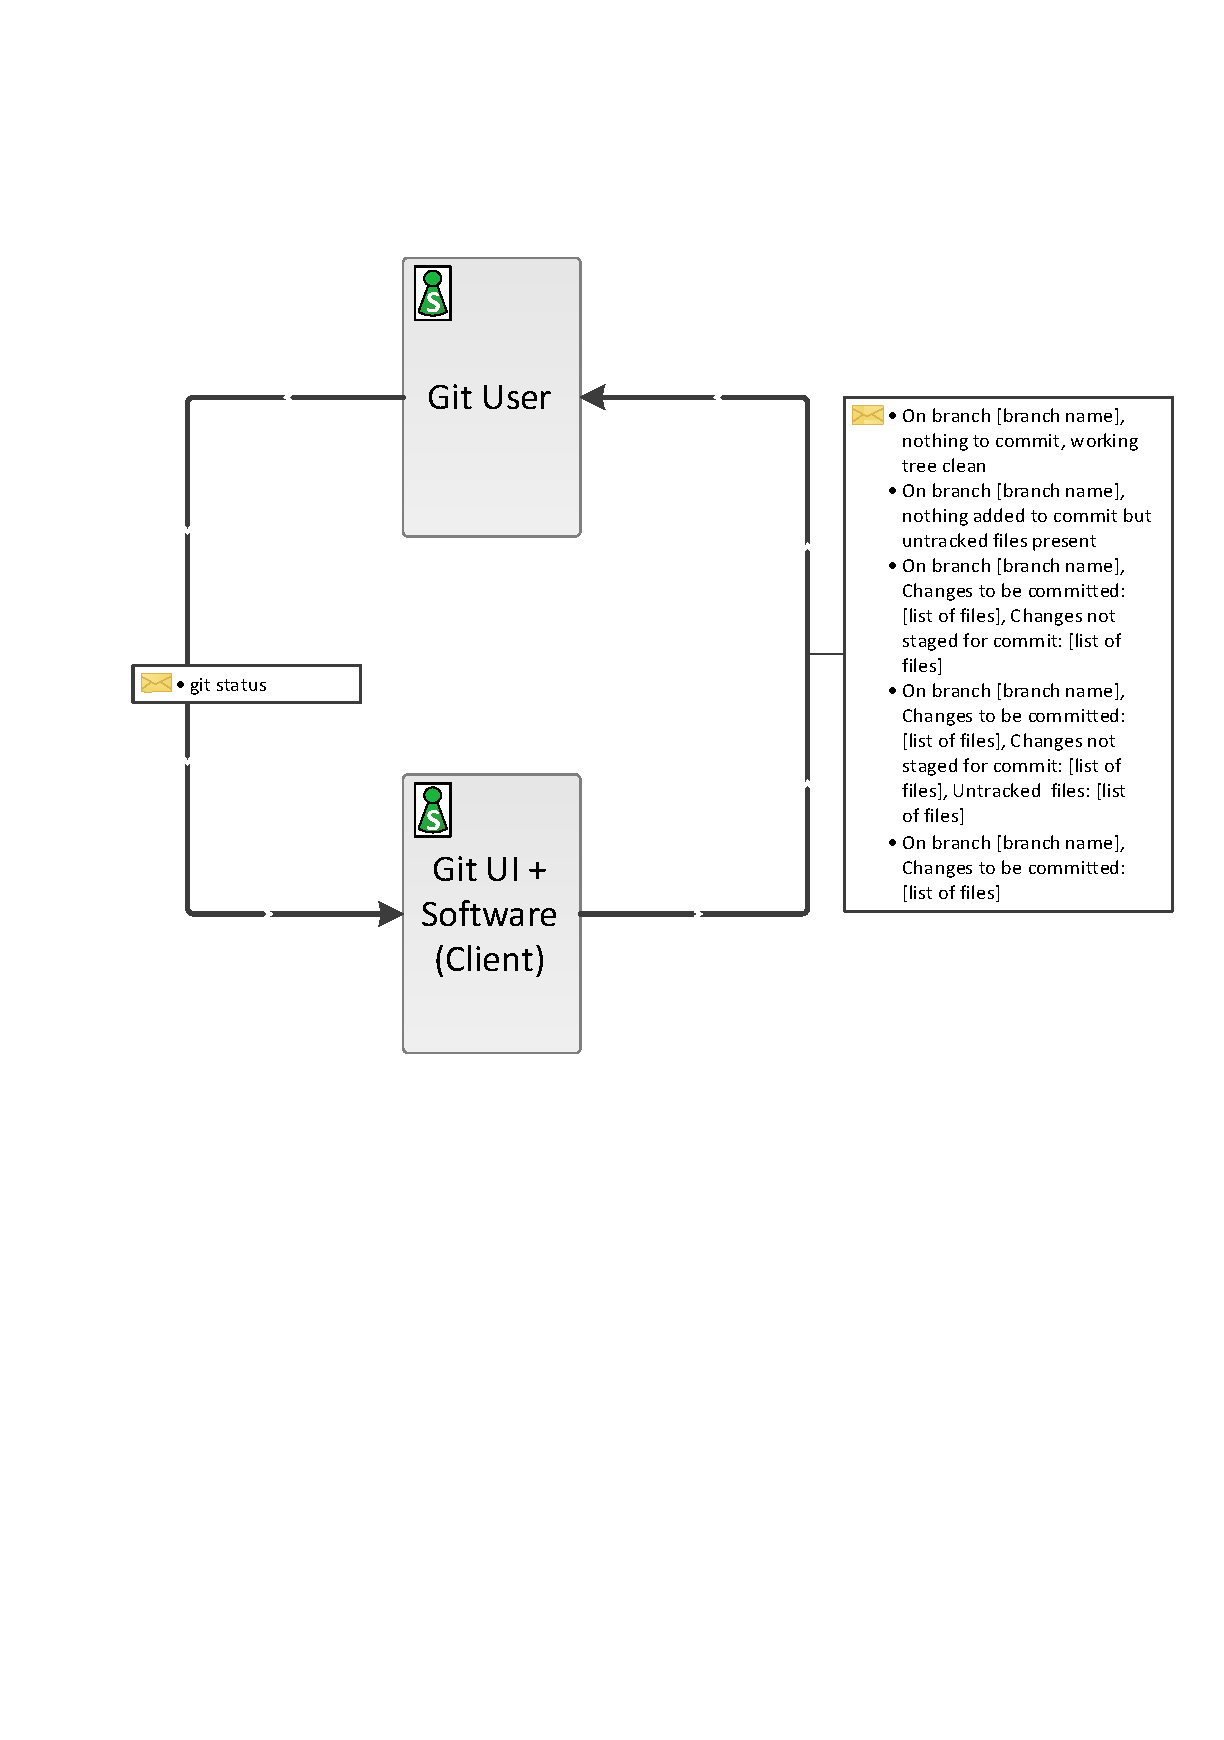
\includepdf[pages=1,pagecommand= {\section{git status} \label{sec:git_status} \subsection{git status local}},scale=0.9]{git_commands/git_status_local.pdf}
\includepdf[pages=2,pagecommand={} ,scale=0.78, angle = 270]{git_commands/git_status_local.pdf}
\includepdf[pages=3,pagecommand={} ,scale=0.75]{git_commands/git_status_local.pdf}
\newpage

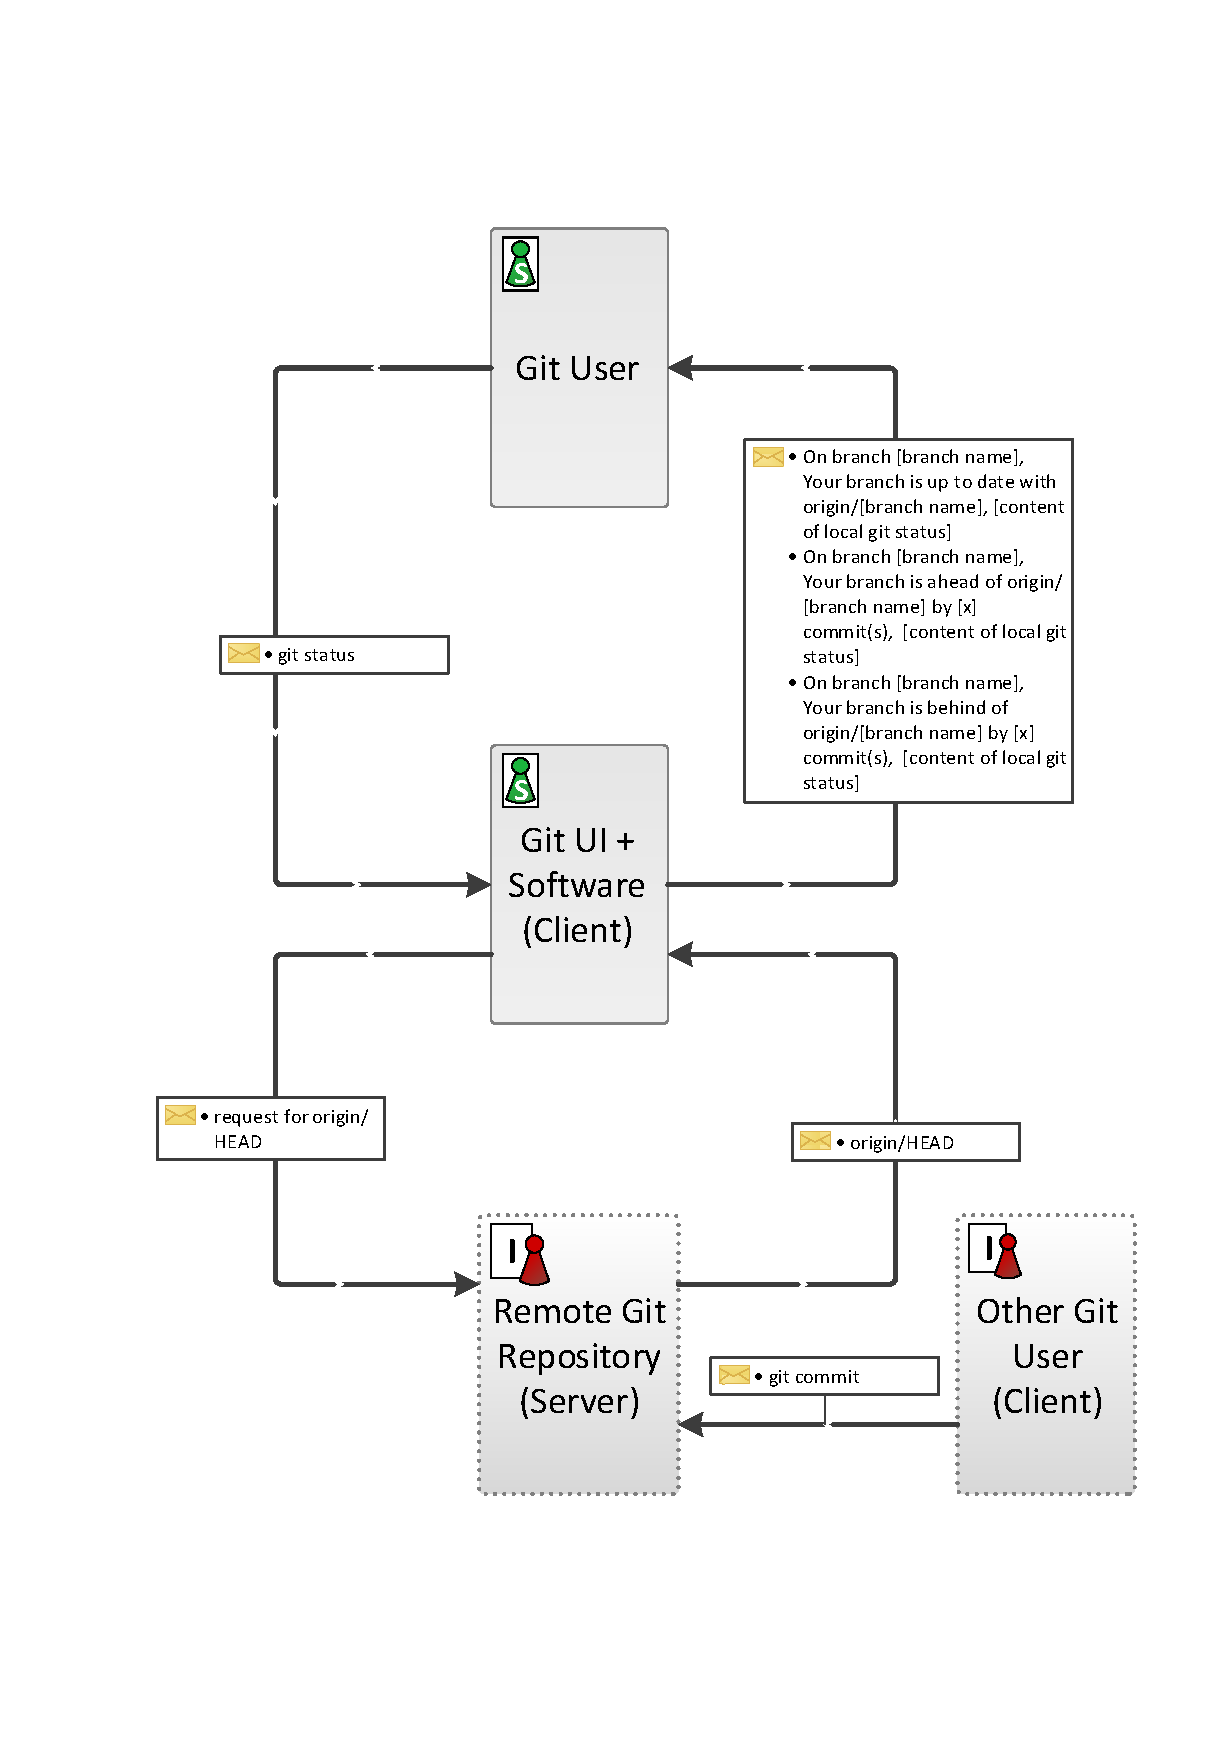
\includepdf[pages=1,pagecommand= {\subsection{git status remote}},scale=0.72]{git_commands/git_status_remote.pdf}
\includepdf[pages=2-last,pagecommand={} ,scale=0.75]{git_commands/git_status_remote.pdf}
\chapter{Git Branching}
\label{cha:git_branching}
This chapter focuses on the git commands which are responsible for creating and switching between diverging versioning timelines. The timelines can be worked on independently from each other. These diverging versioning timelines are called \dq{}branches\dq{}. After finishing this chapter, the reader is able to view all existing branches, checkout any existing branch, merge different branches and set a new beginning point for any branch.

\textit{Additional Information}: Every branch has a branch-pointer. This pointer points at the latest commit of the given branch. The main difference between the branch-pointer and the HEAD (defined in \nameref{cha:git_basics}) is that the HEAD is actually pointing at the branch-pointer of the current branch. Thus, the HEAD is only indirectly pointing at the latest commit which is dependent on the current branch, as seen in (\ref{fig:branch_pointer}).
Every git repository has a \dq{}master\dq{} branch. This branch is the main branch from which all other branches may originate.
\begin{figure}[H]
    \centering
    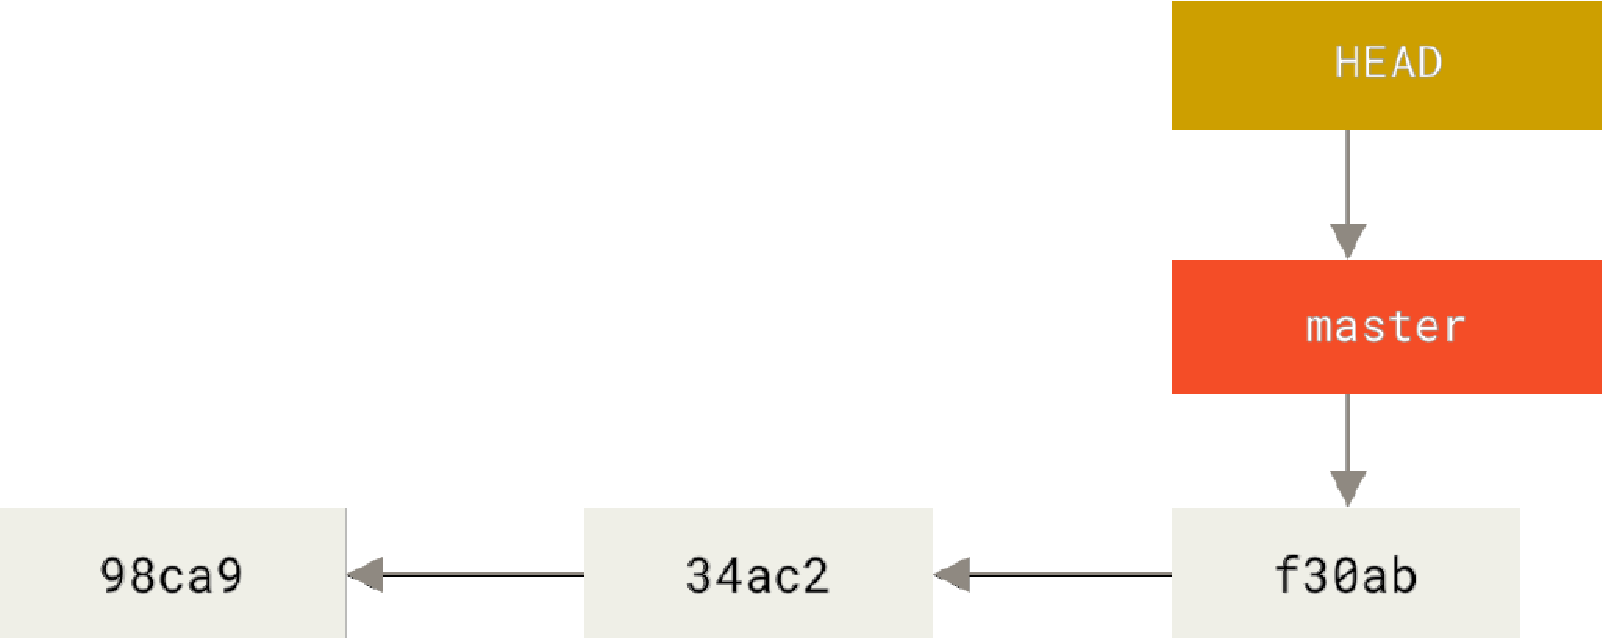
\includegraphics[width=\textwidth]{git_manual/figures/branch_pointer.pdf}
    \caption{The master branch pointer points at the latest commit. The HEAD points at the current branch which is the master \cite{CS20}.}
    \label{fig:branch_pointer}
\end{figure}

\newpage

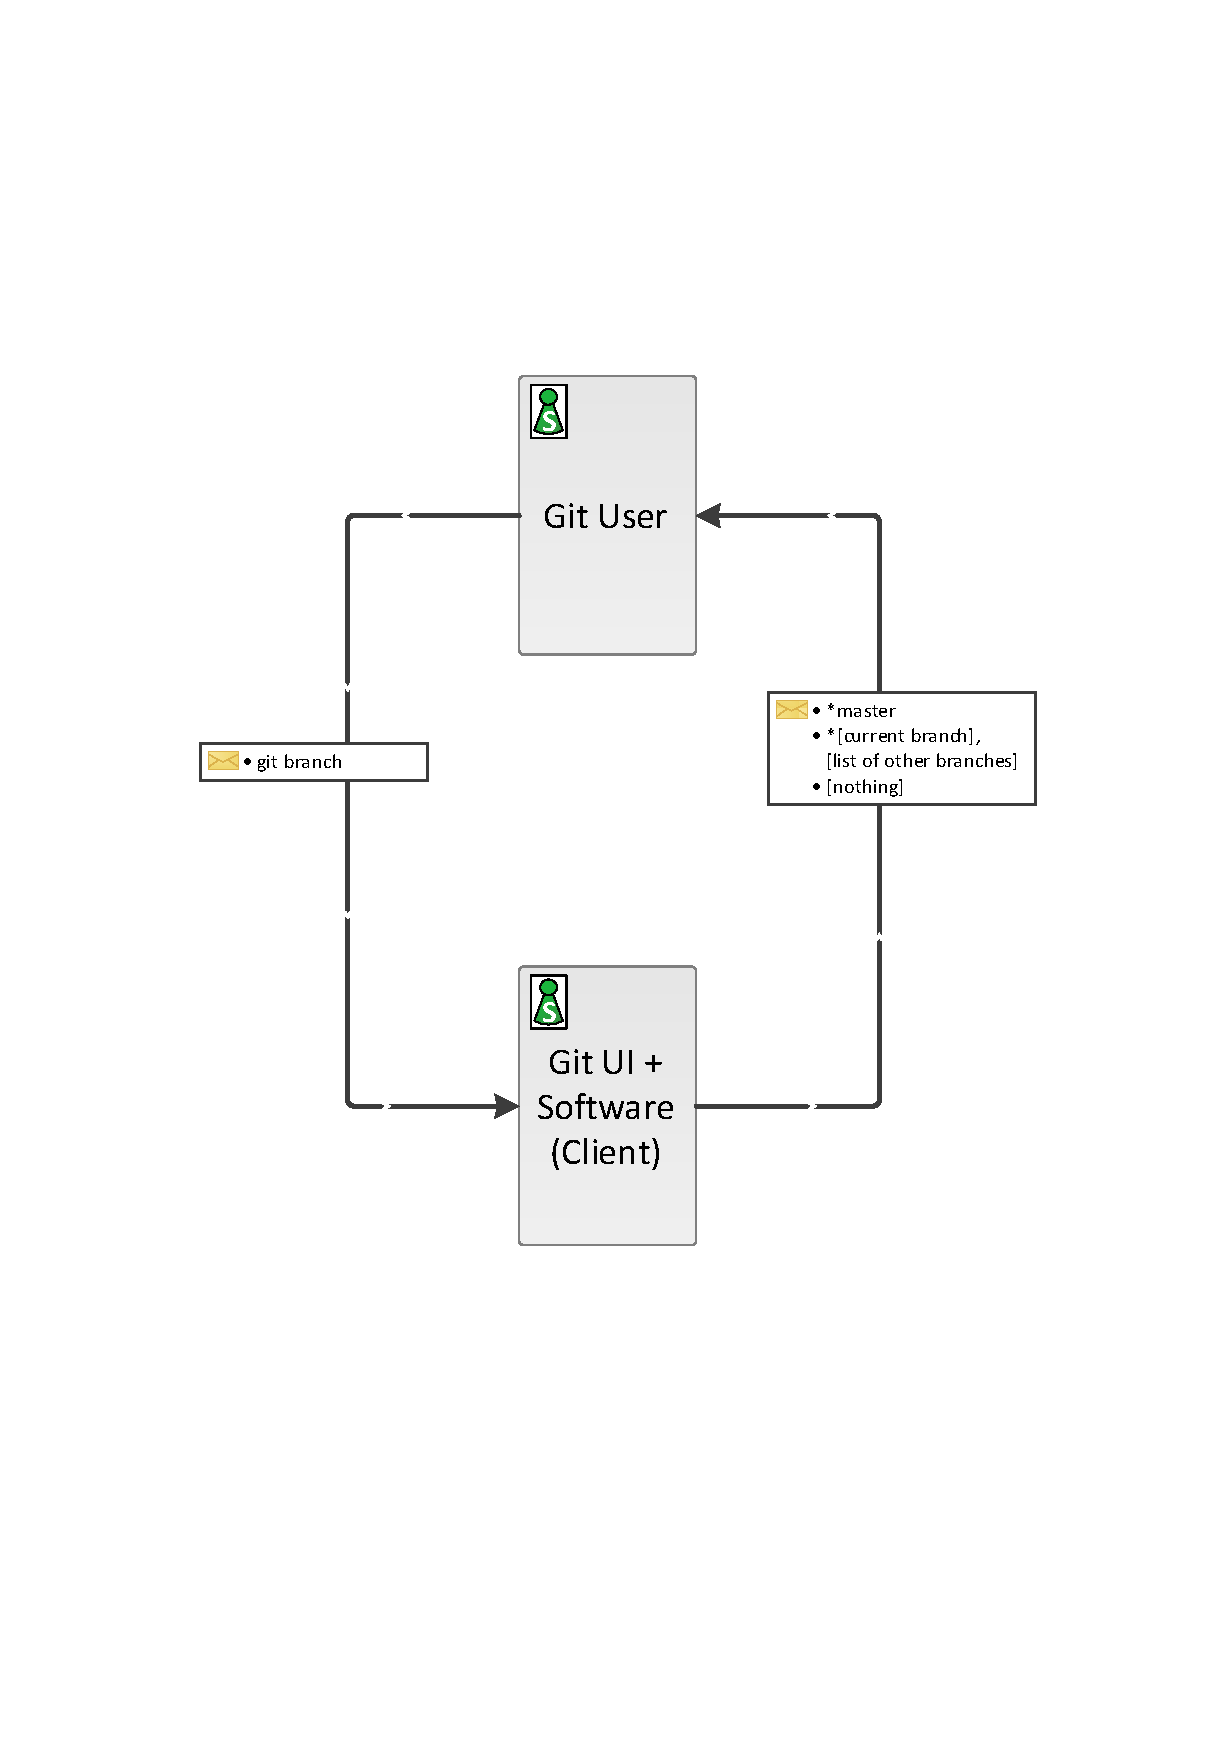
\includepdf[pages=1,pagecommand= {\section{git branch} \label{sec:git_branch} \subsection{git branch}},scale=0.9]{git_commands/git_branch.pdf}
\includepdf[pages=2-last,pagecommand={} ,scale=0.75]{git_commands/git_branch.pdf}

\newpage

\includepdf[pages=1,pagecommand= {\subsection{git branch [name]}},scale=0.9]{git_commands/git_branch_name.pdf}
\includepdf[pages=2-last,pagecommand={} ,scale=0.75]{git_commands/git_branch_name.pdf}

\newpage

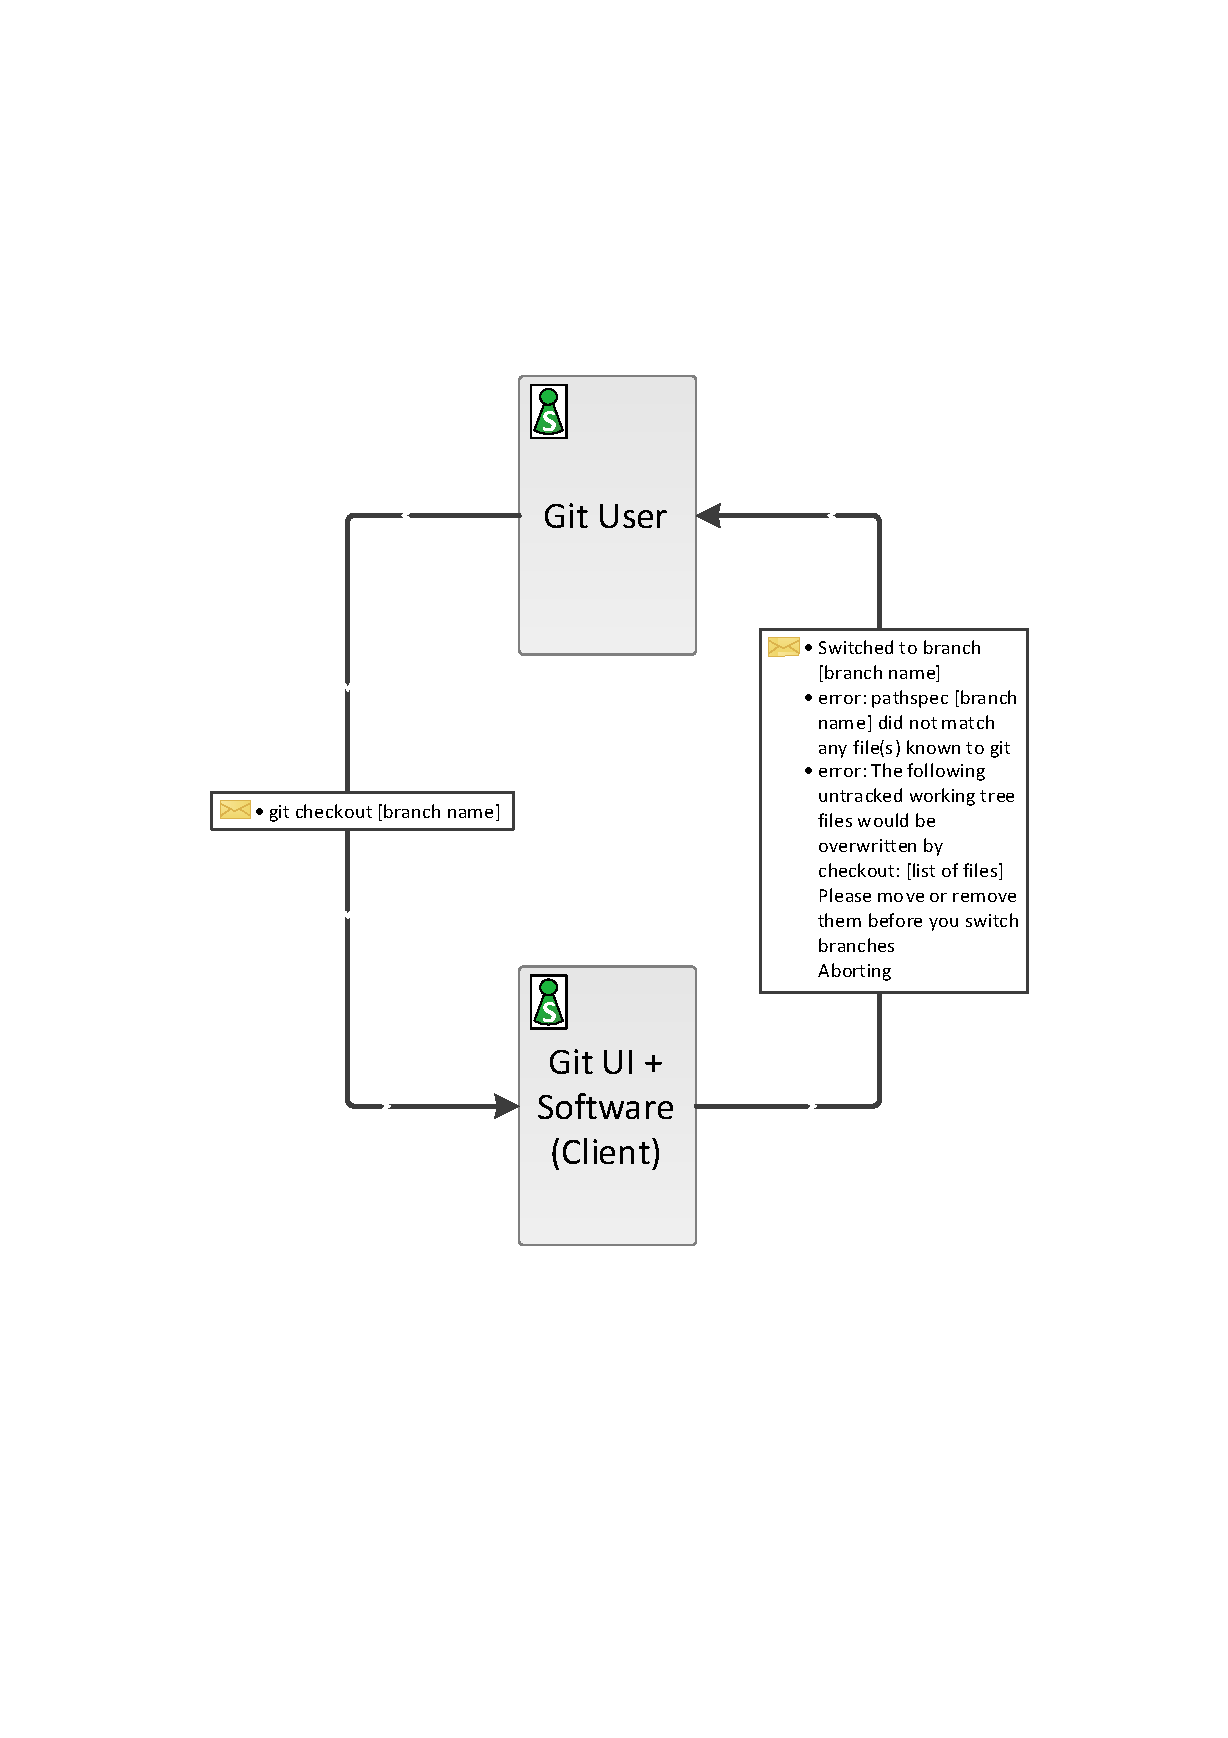
\includepdf[pages=1,pagecommand= {\section{git checkout} \label{sec:git_checkout}},scale=0.9]{git_commands/git_checkout.pdf}
\includepdf[pages=2-last,pagecommand={} ,scale=0.75]{git_commands/git_checkout.pdf}

\newpage

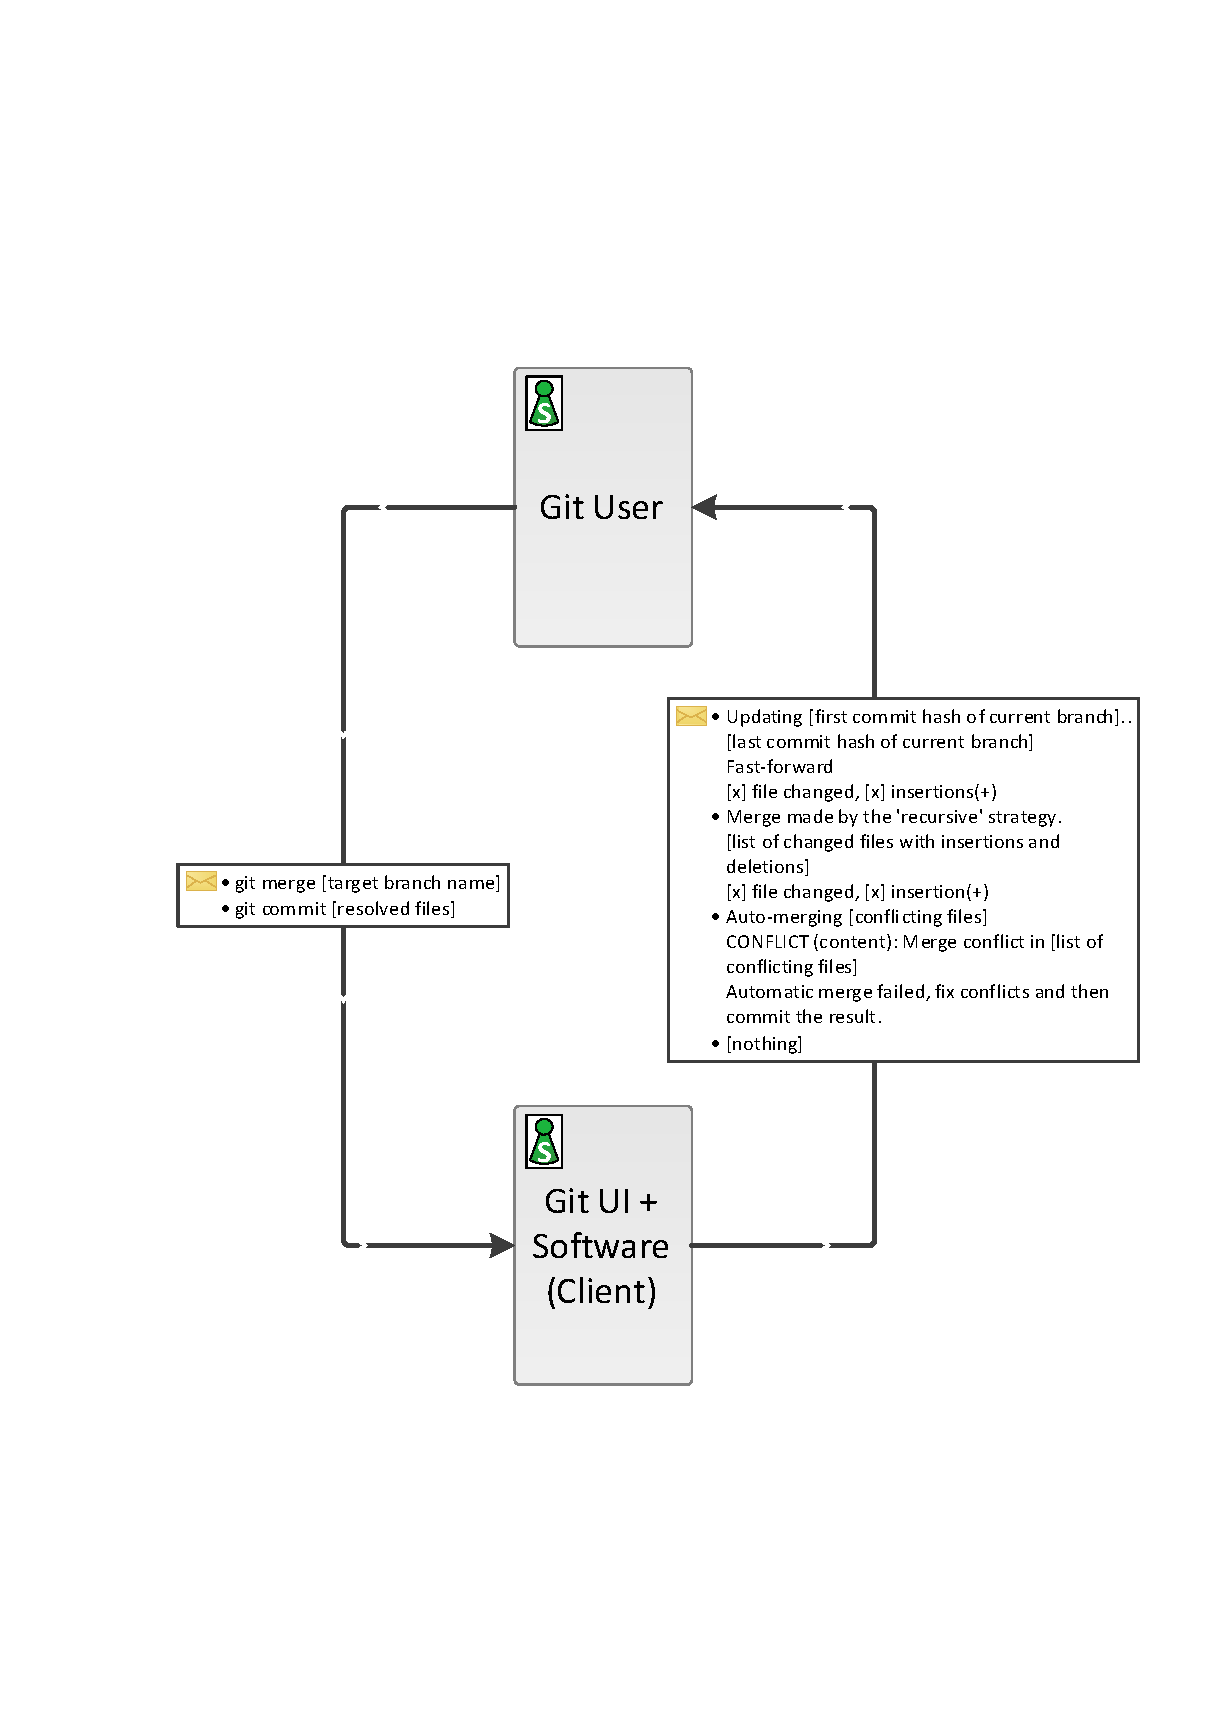
\includepdf[pages=1,pagecommand= {\section{git merge} \label{sec:git_merge}} ,scale=0.9]{git_commands/git_merge.pdf}
\includepdf[pages=2-last,pagecommand={} ,scale=0.75]{git_commands/git_merge.pdf}

\newpage

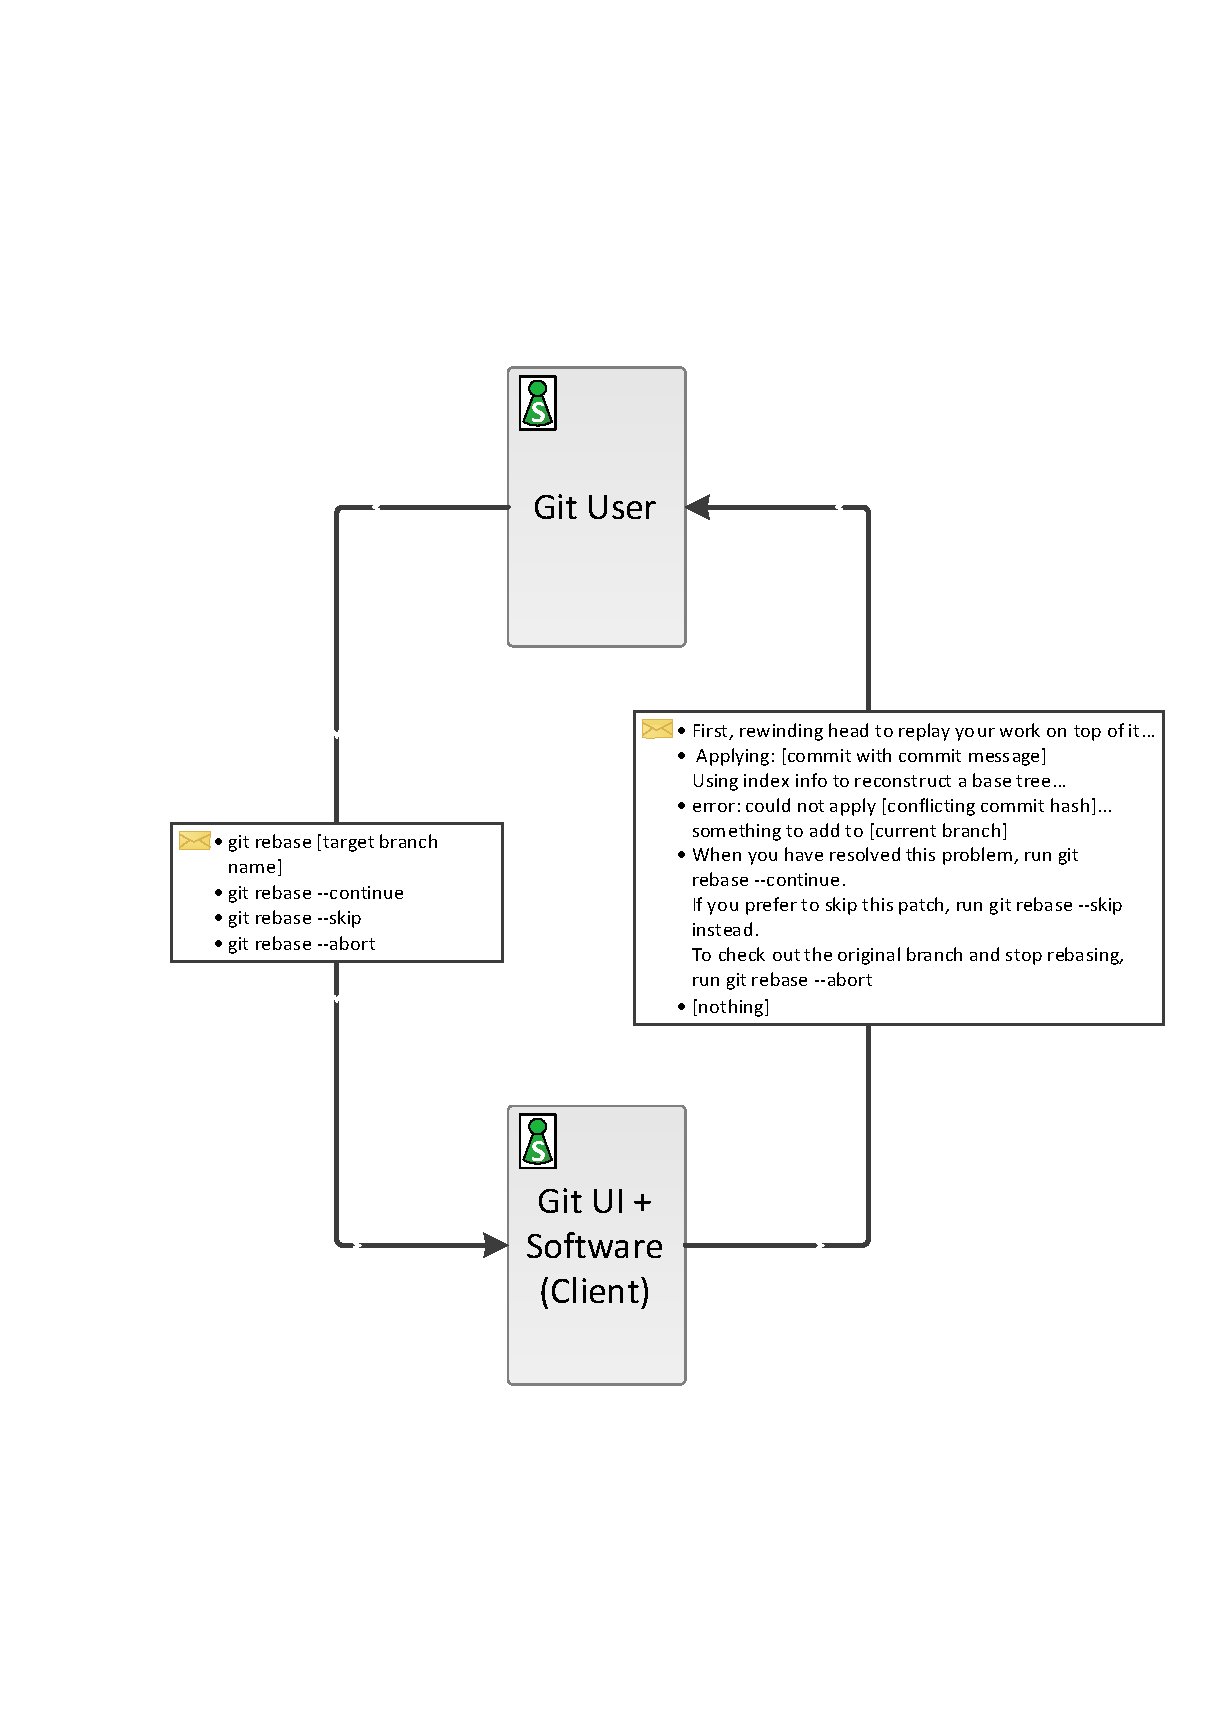
\includepdf[pages=1,pagecommand= {\section{git rebase} \label{sec:git_rebase}} ,scale=0.9]{git_commands/git_rebase.pdf}
\includepdf[pages=2,pagecommand={} ,scale=0.8]{git_commands/git_rebase.pdf}
\includepdf[pages=last,pagecommand={} ,scale=0.81]{git_commands/git_rebase.pdf}
\chapter{Git Collaborations}
\label{cha:git_collaboration}
This chapter contains every git command that is related to working on and with remote repositories. Thus, every command in this chapter requires a network connection to work. After finishing this chapter, the reader will be able to clone a remote repository, fetch all the existing branches and commits of that remote repository, pull additional commits from the remote repository and push new commits to the remote repository.

\newpage

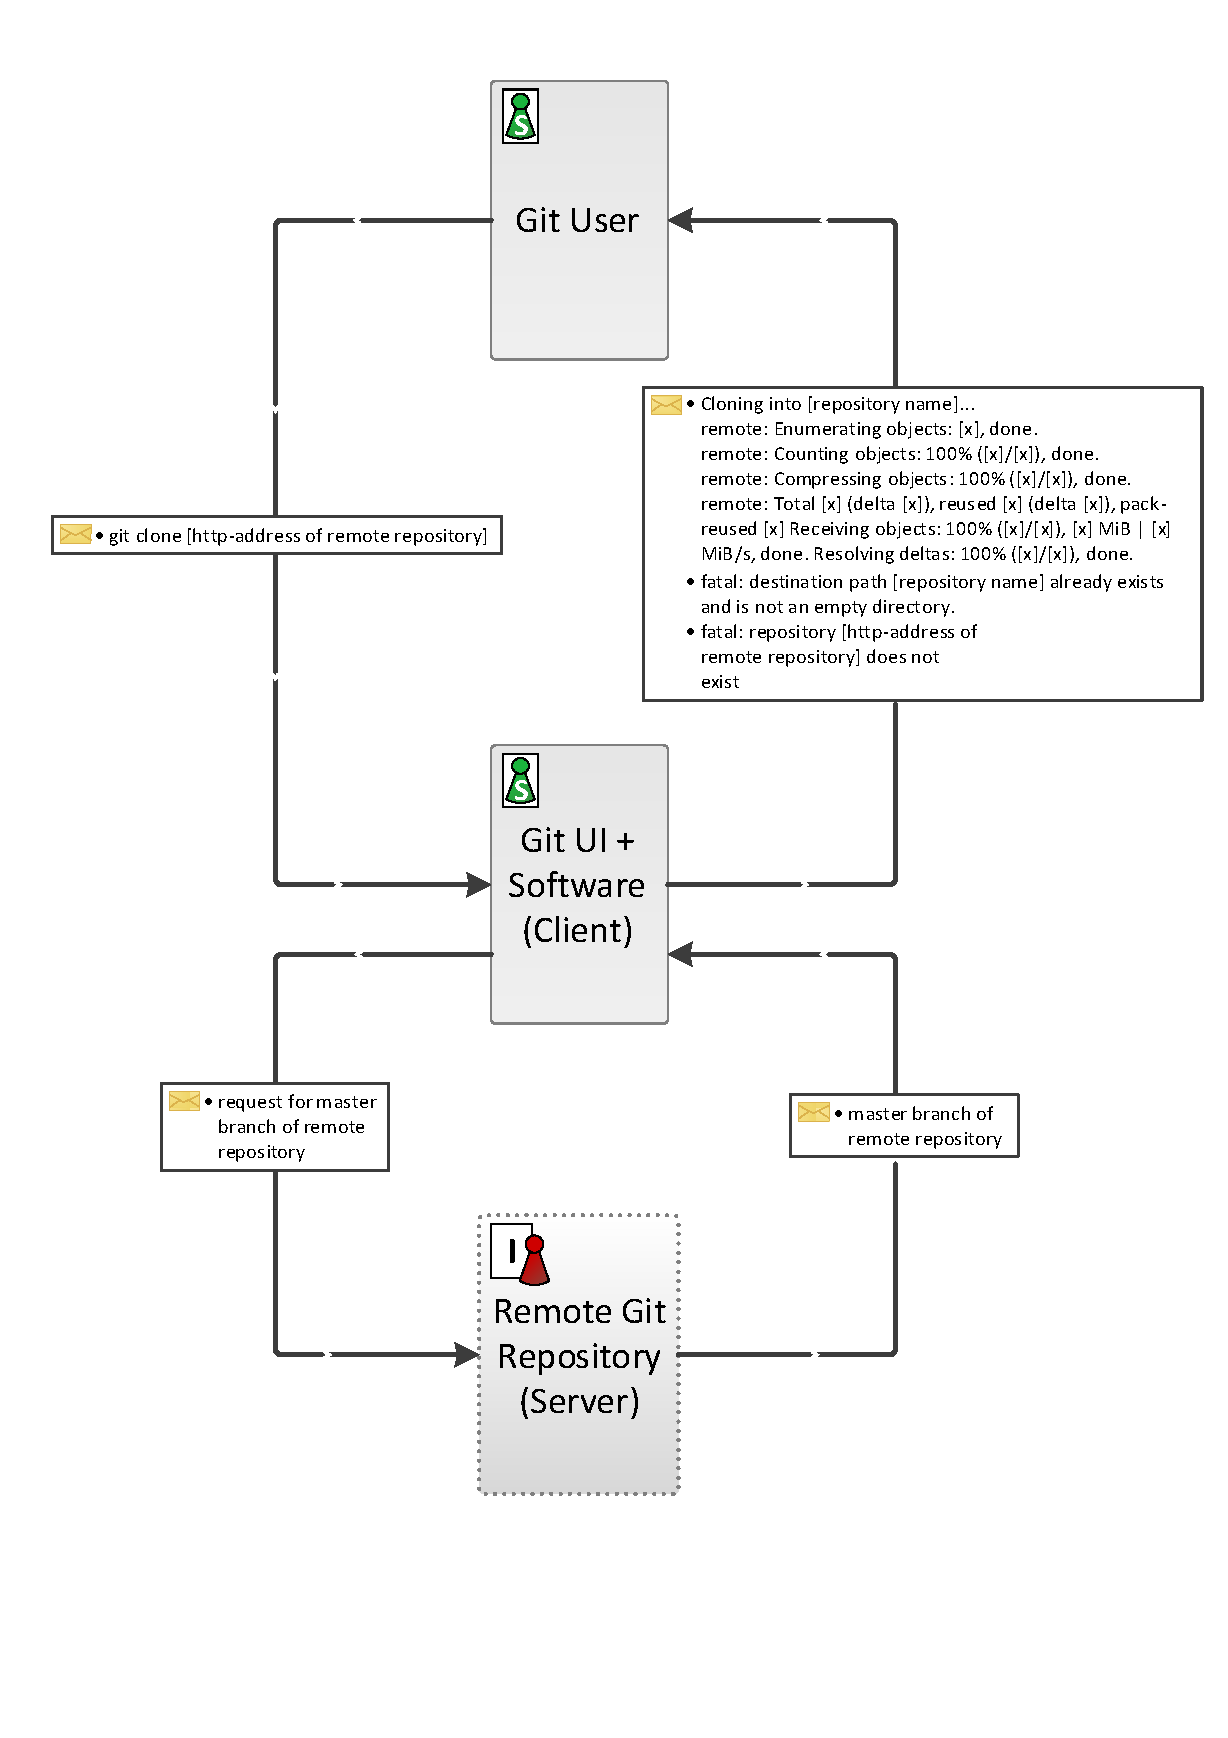
\includepdf[pages=1,pagecommand= {\section{git clone} \label{sec:git_clone}},scale=0.72]{git_commands/git_clone.pdf}
\includepdf[pages=2-last,pagecommand={} ,scale=0.75]{git_commands/git_clone.pdf}

\newpage

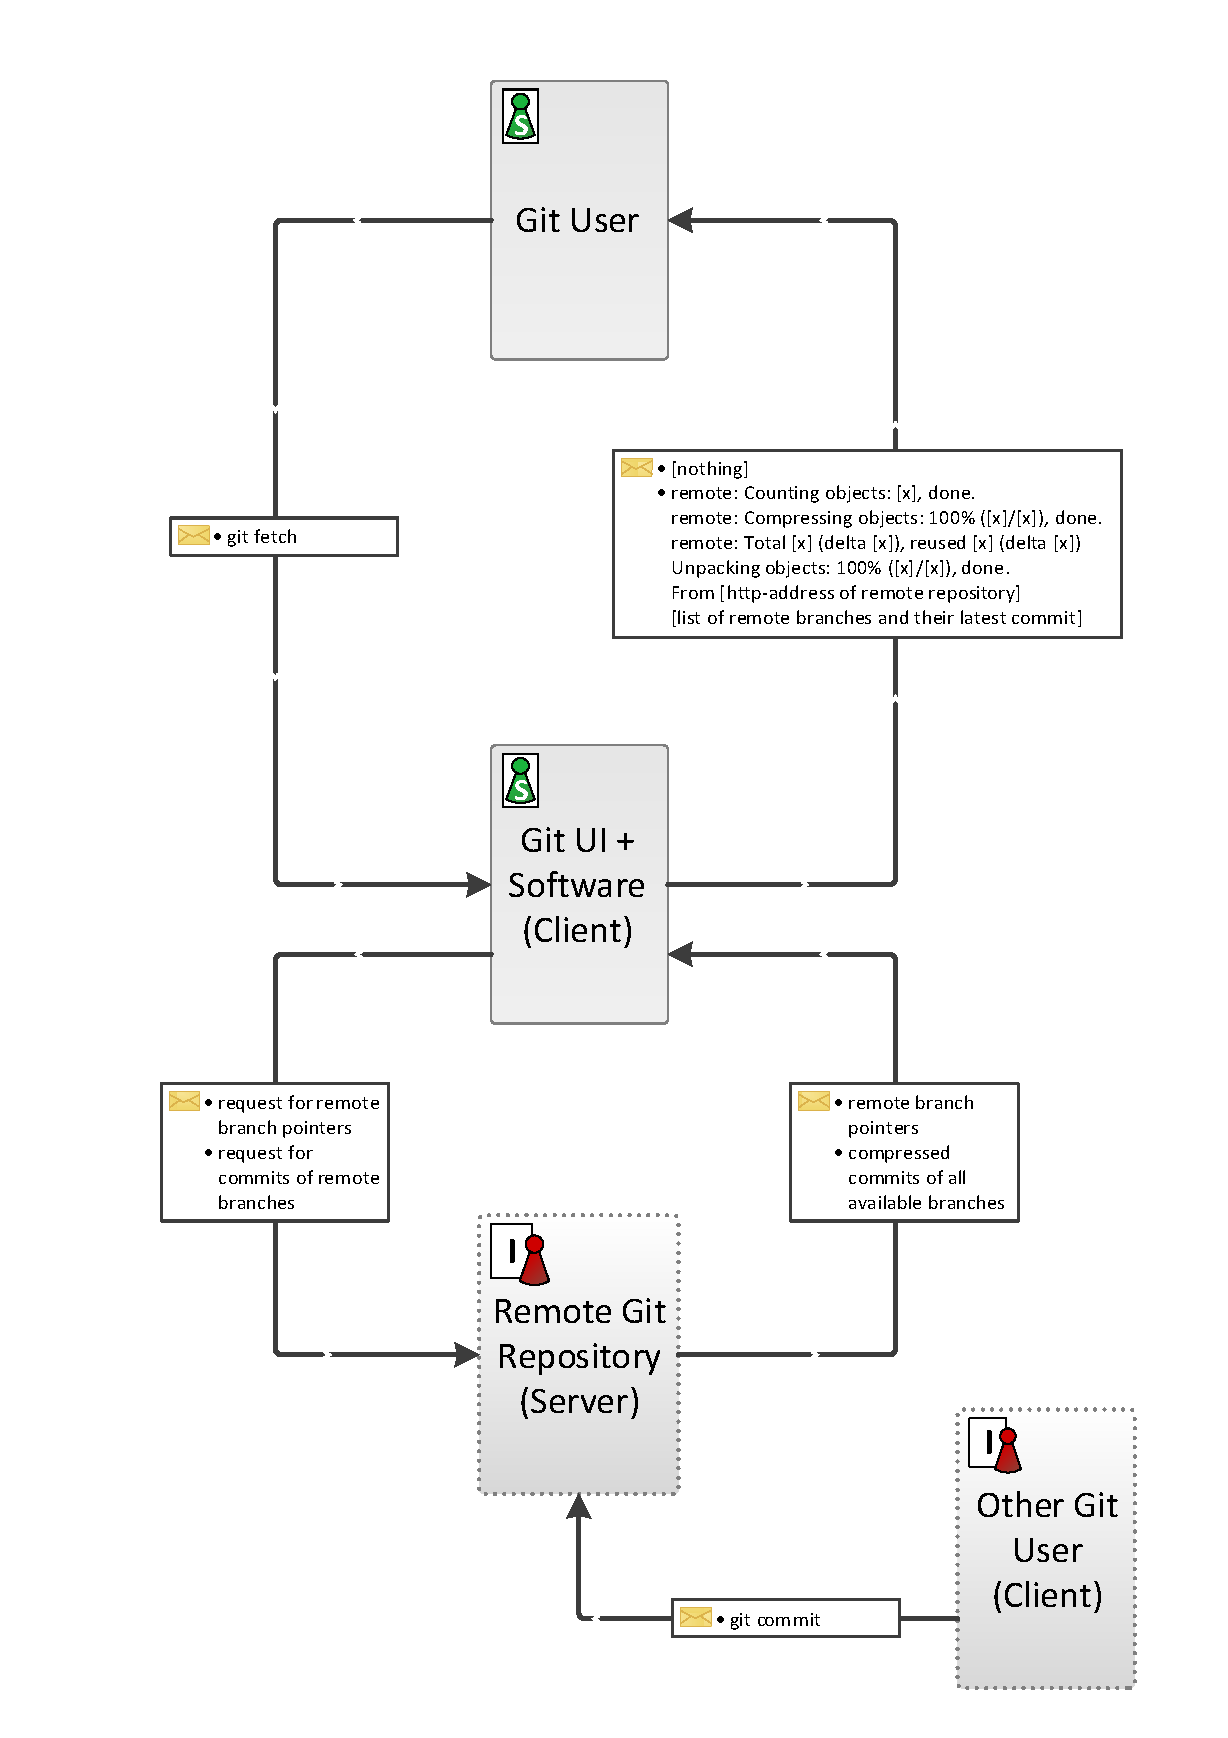
\includepdf[pages=1,pagecommand= {\section{git fetch} \label{sec:git_fetch}},scale=0.72]{git_commands/git_fetch.pdf}
\includepdf[pages=2-last,pagecommand={} ,scale=0.75]{git_commands/git_fetch.pdf}

\newpage

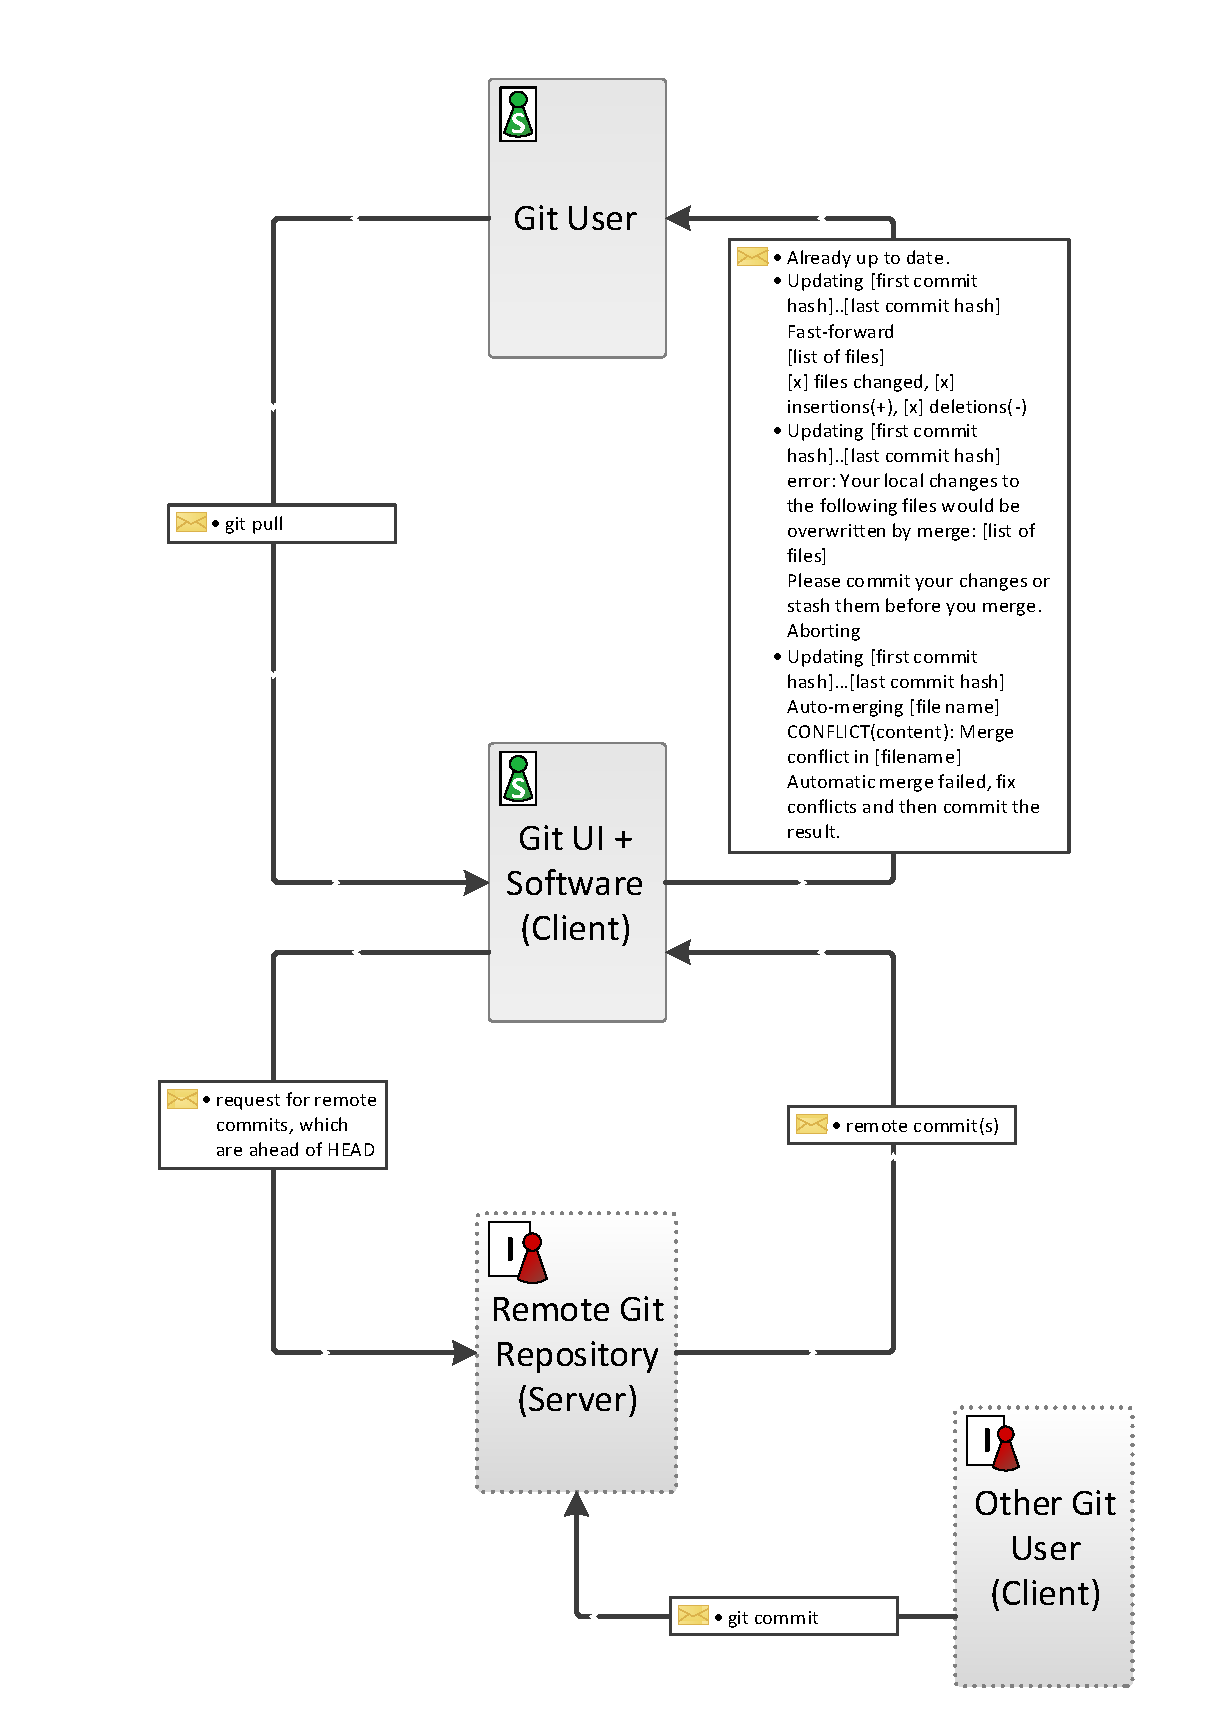
\includepdf[pages=1,pagecommand= {\section{git pull} \label{sec:git_pull}} ,scale=0.72]{git_commands/git_pull.pdf}
\includepdf[pages=2-last,pagecommand={} ,scale=0.75]{git_commands/git_pull.pdf}

\newpage

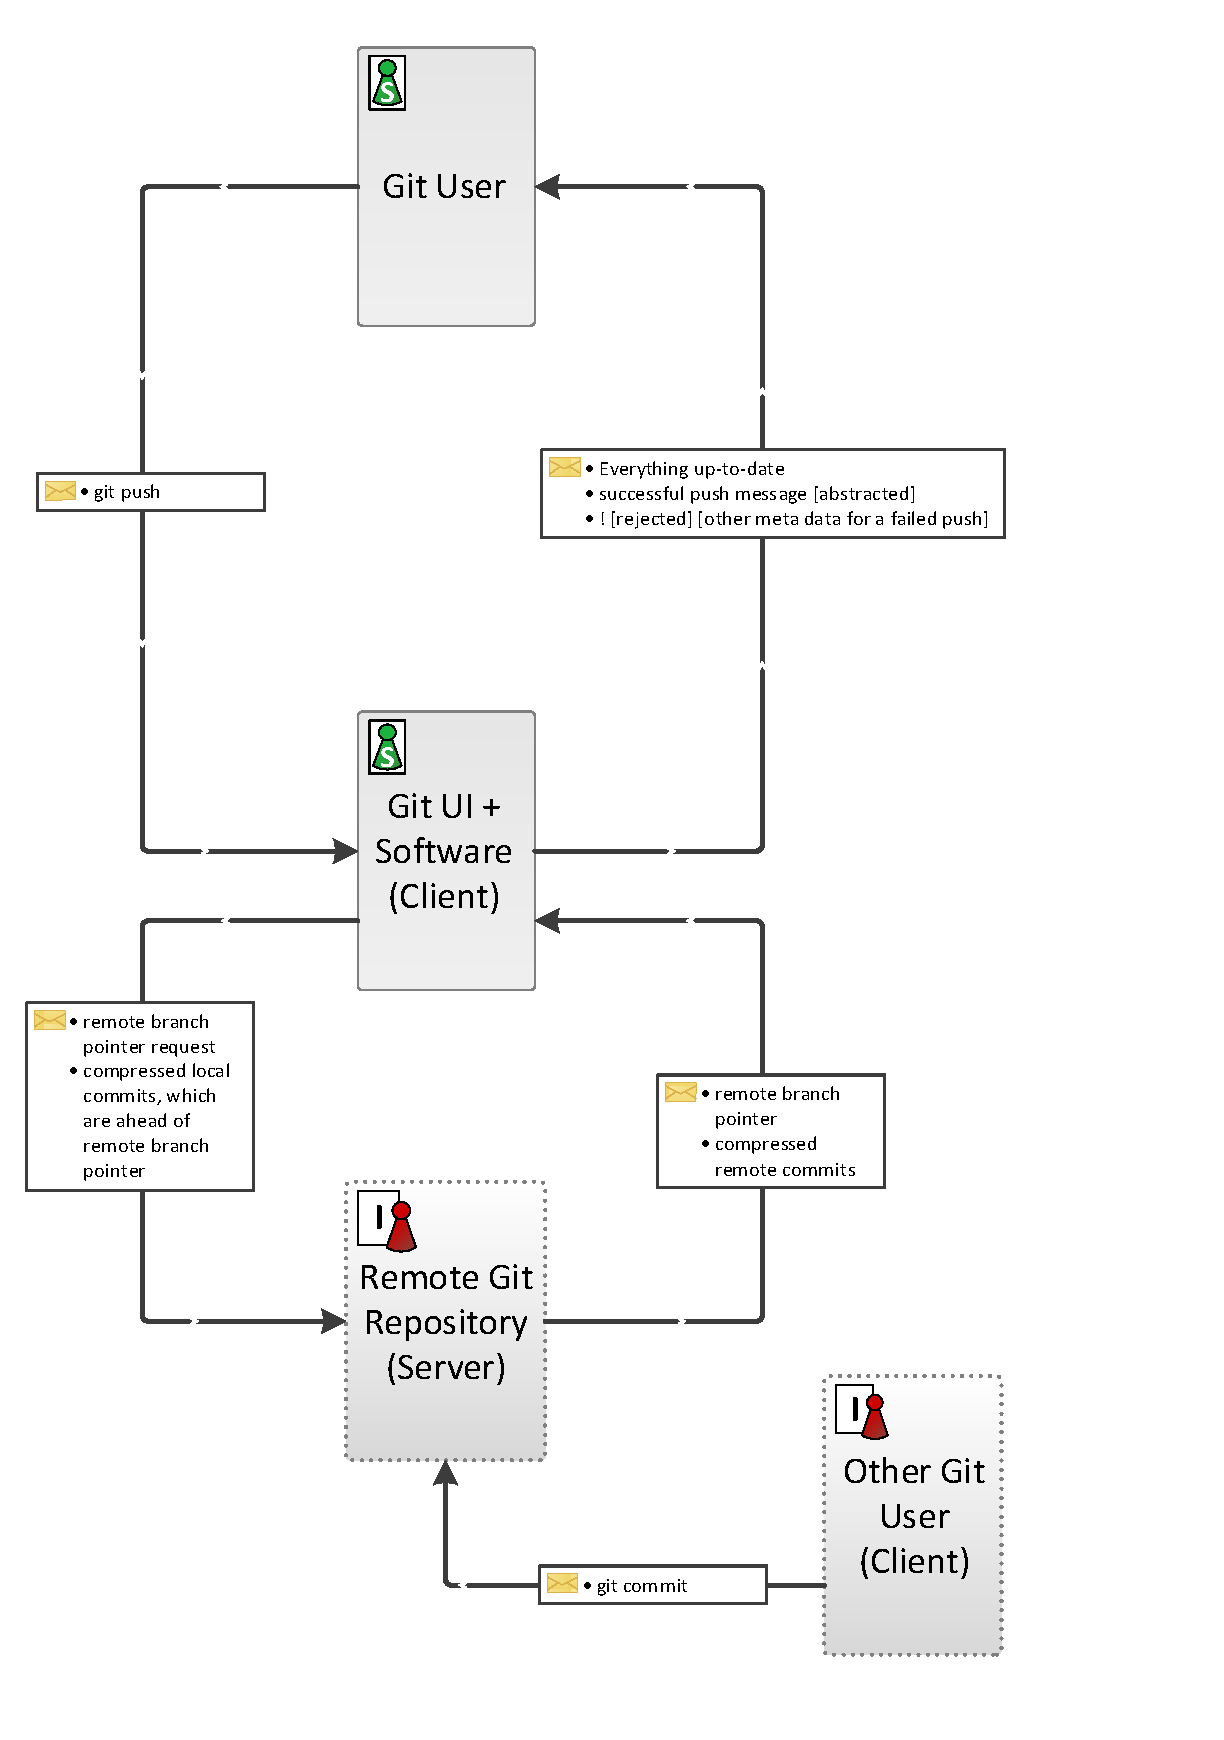
\includepdf[pages=1,pagecommand= {\section{git push} \label{sec:git_push}} ,scale=0.72]{git_commands/git_push.pdf}
\includepdf[pages=2-last,pagecommand={} ,scale=0.8]{git_commands/git_push.pdf}

%
% add appendix
%

\chapter{Appendix}
\chaptermark{Appendix}


\bibliography{name_sepr}

\bibliographystyle{cmnat}
%\includepdf[pages=2-last, pagecommand={\thispagestyle{scrheadings}}, scale=0.7]{chapters/anhang.pdf}
%\includepdf[pages=1, pagecommand={\section{Final Presentation in the WASA Lecture} \thispagestyle{scrheadings}}, scale=0.7]{attachment/cm-teamarbeit.pdf}
%\includepdf[pages=1, pagecommand={\thispagestyle{scrheadings}}, scale=0.7]{attachment/cm-teamarbeit2.pdf}
%\includepdf[pages=2, pagecommand={\thispagestyle{scrheadings}}, scale=0.7]{attachment/cm-teamarbeit2.pdf}


%
% Abbreviations
%

\setglossarysection{section}
\setglossarystyle{alttree}
\glssetwidest{SAMPLETE}
\printglossary[numberedsection, nonumberlist, type=\acronymtype, title=Abbreviations]
%\clearpage
\chaptermark{Appendix}

%
% Bibliography
%

\makeatletter
\renewenvironment{thebibliography}[1]
     {\section{\bibname}
           \list{\@biblabel{\@arabic\c@enumiv}}
           {\settowidth\labelwidth{\@biblabel{#1}}
            \leftmargin\labelwidth
            \advance\leftmargin\labelsep
            \@openbib@code
            \usecounter{enumiv}%
            \let\p@enumiv\@empty
            \renewcommand\theenumiv{\@arabic\c@enumiv}}
      \sloppy
      \clubpenalty4000
      \@clubpenalty \clubpenalty
      \widowpenalty4000
      \sfcode`\.\@m}
     {\def\@noitemerr
       {\@latex@warning{Empty `thebibliography' environment}}%
      \endlist}
\makeatother




%==============================================================================

\end{document}